\subsection{MANEUVERS}

\begin{tcoloritemize}
    \blueitem[Tactical Turn]
    \textbf{Maintains LAB formation} --- flight member on outside must initiate turn
    
    \hfill\textbf{Reference \cref{fig:supp_fig:form:tacturn}}

    \blueitem[Hook Turn]
    \textbf{Element turns cold while maintaining LAB} --- ideal for CAP / grinder tactics
    
    \hfill\textbf{Reference \cref{fig:supp_fig:form:hookturn}}

    \blueitem[Cross Turn]
    \textbf{Element turns cold while maintaining LAB} --- similar to hook turn, flight members swap sides
    
    \hfill\textbf{Reference \cref{fig:supp_fig:form:crossturn}}

    \blueitem[Shackle]
    \textbf{Element members swap sides}
    
    \hfill\textbf{Reference \cref{fig:supp_fig:form:shackle}}

    \blueitem[In-Place Turn]
    \textbf{Places wingman in trail} --- can be combined with 2nd in-place turn to return to LAB

    \hfill\textbf{Reference \cref{fig:supp_fig:form:inplace}}
\end{tcoloritemize}

\begin{figure}[htbp]
    \centering
    \begin{subfigure}[b]{0.45\linewidth}
        \centering
        \begin{tikzpicture}[figstyle]
            
            \draw[->] 
            (0,0) -- 
            node[below, pos=0]{
                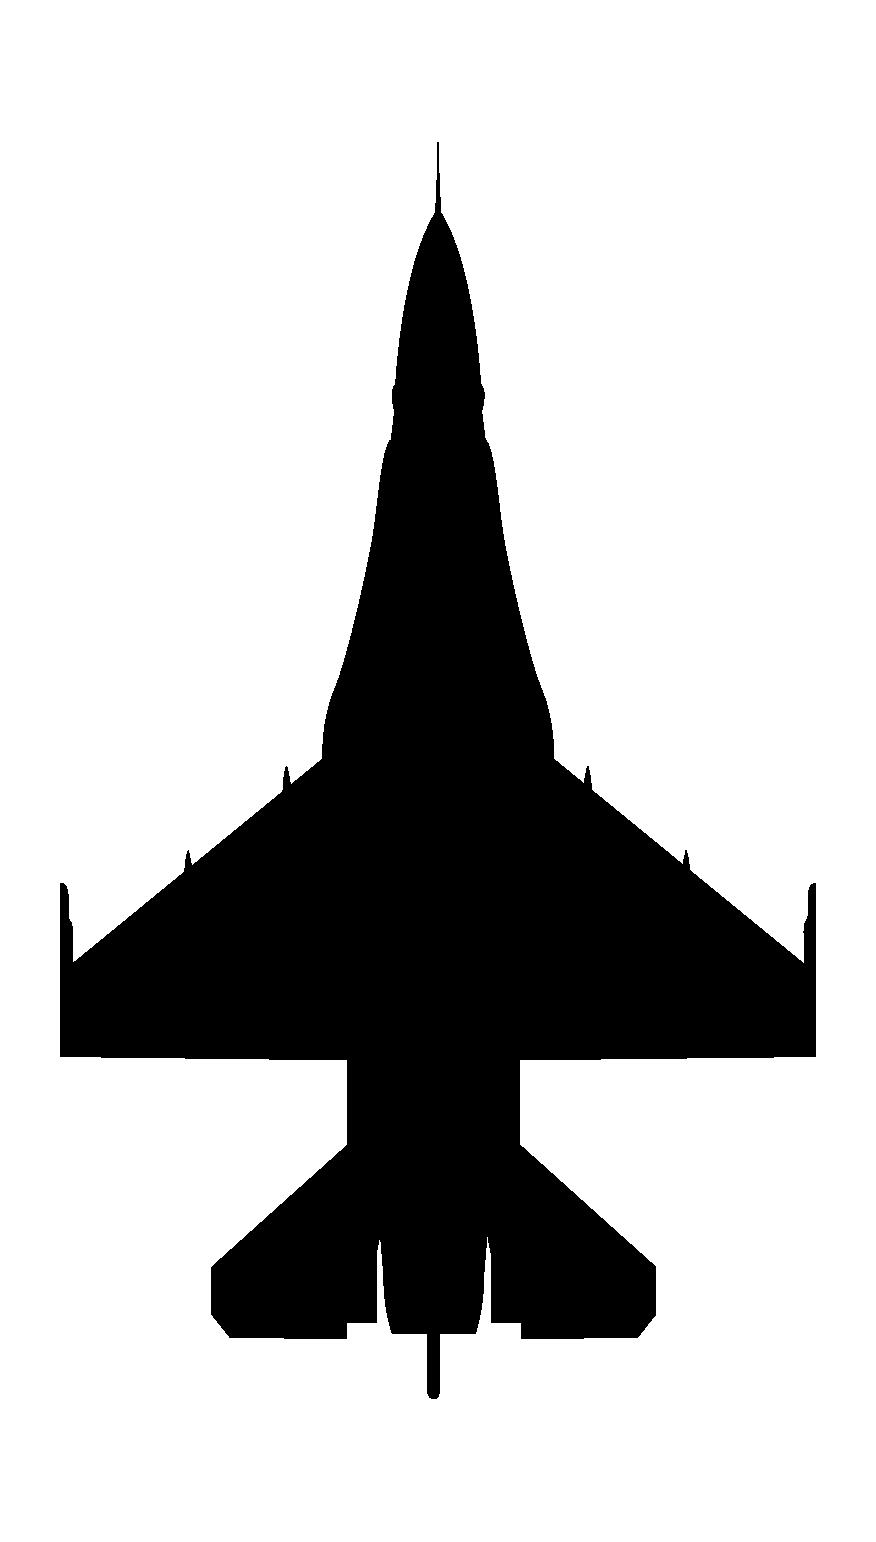
\includegraphics[
                width=7.5mm,
            ]{diagrams/aircraft/silhouette_f16_top.pdf}} 
            ++(0,10) 
            arc (180:90:10) 
            -- ++(20,0) 
            node[above, pos=1, rotate=-90]{
                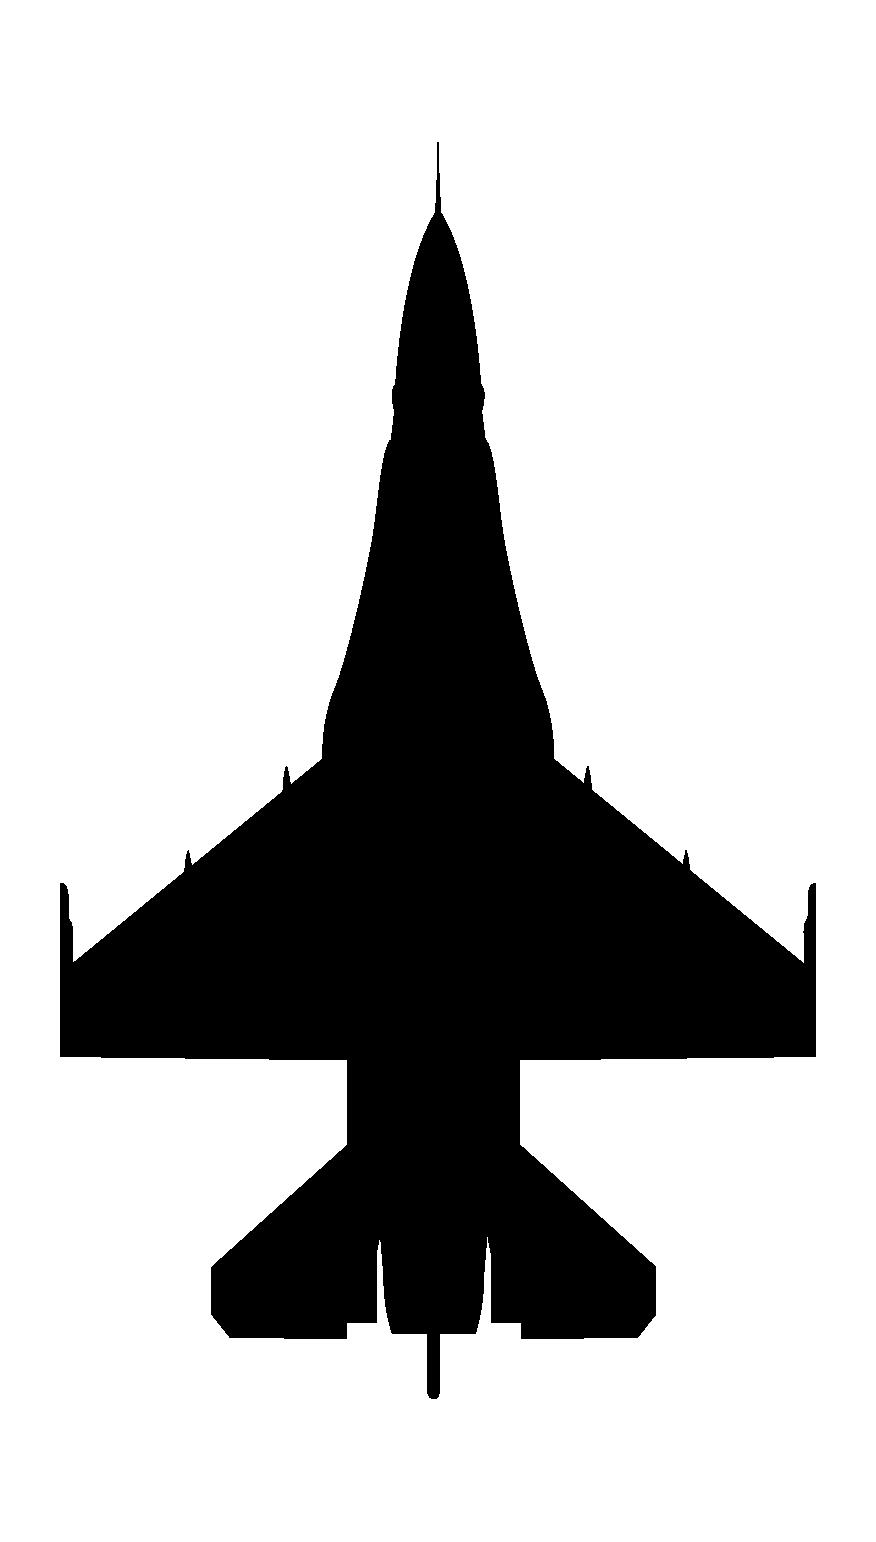
\includegraphics[
                    width=7.5mm,
            ]{diagrams/aircraft/silhouette_f16_top.pdf}};
                
            \draw[->] 
            (10,0) -- 
            node[below, pos=0]{
                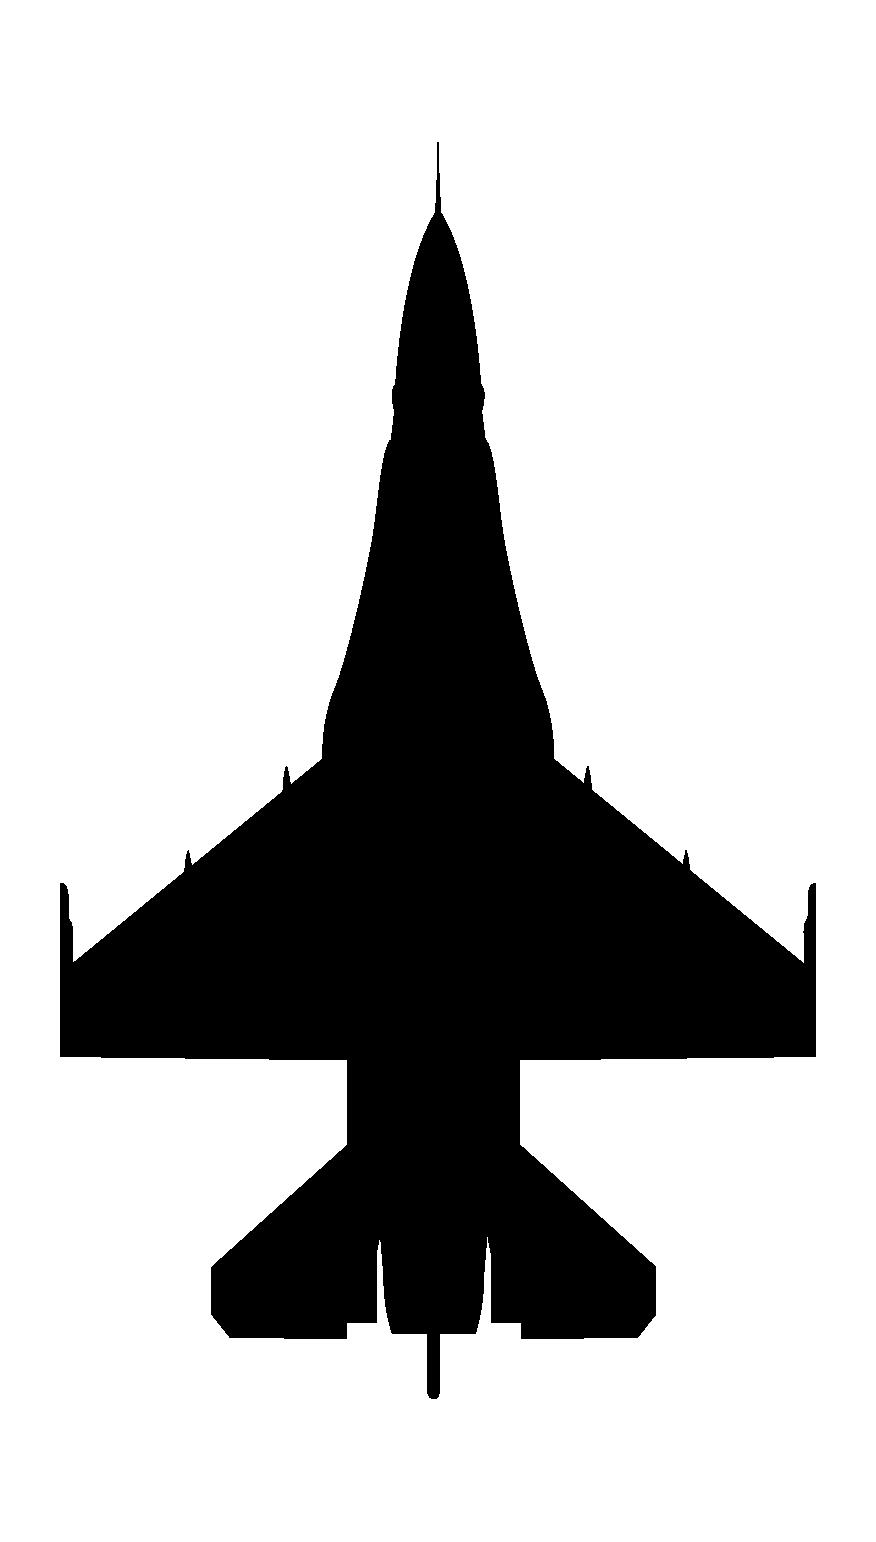
\includegraphics[
                width=7.5mm,
            ]{diagrams/aircraft/silhouette_f16_top.pdf}} 
            ++(0,20) 
            arc (180:90:10) 
            -- ++(10,0) 
            node[above, pos=1, rotate=-90]{
                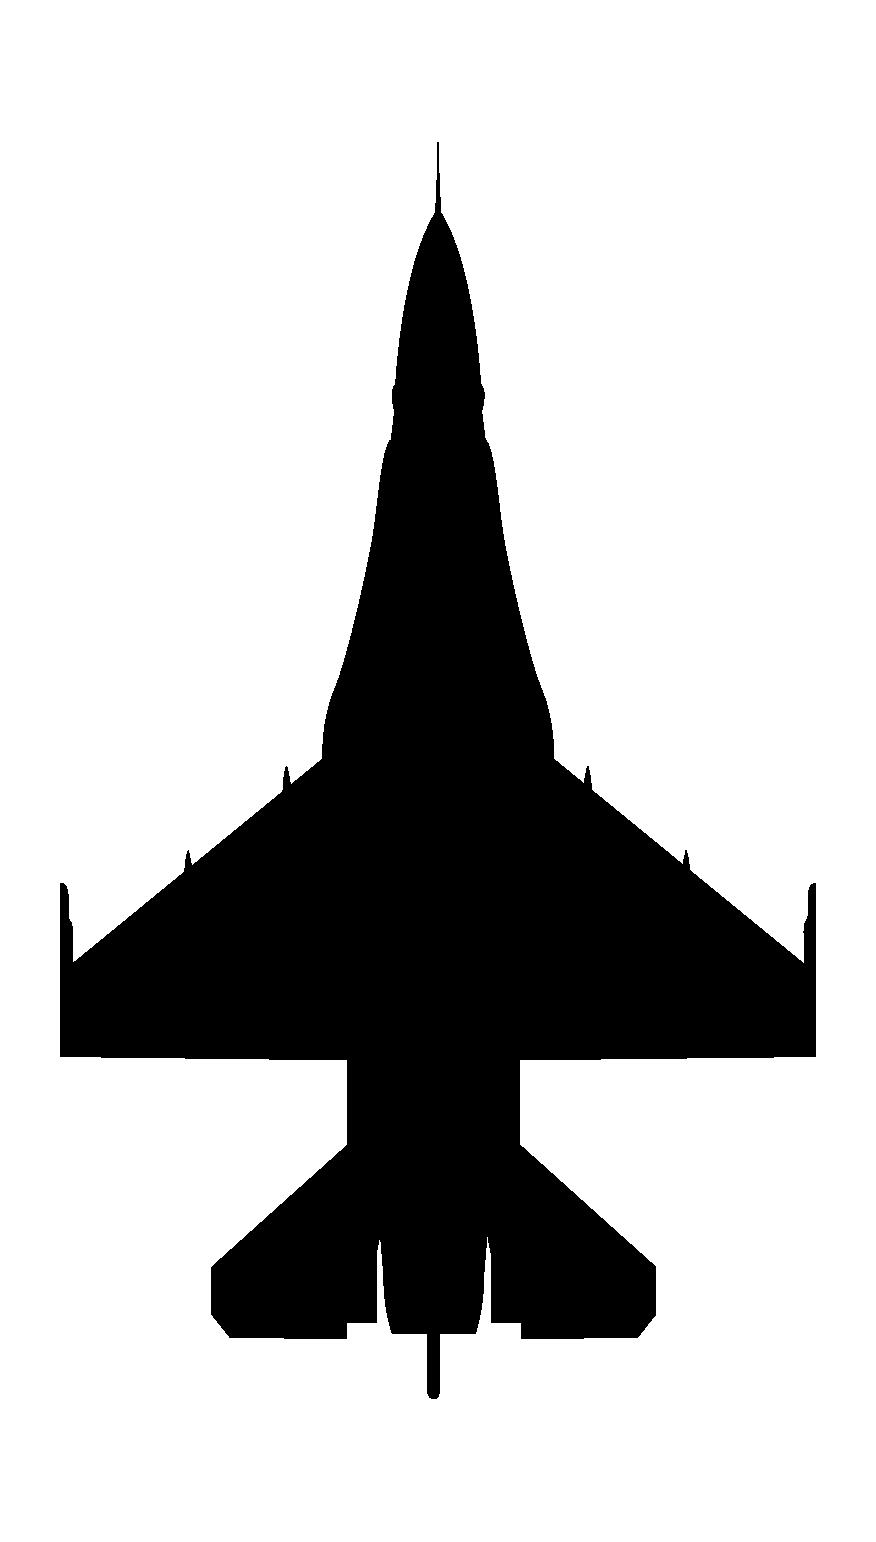
\includegraphics[
                    width=7.5mm,
            ]{diagrams/aircraft/silhouette_f16_top.pdf}};
        \end{tikzpicture}
        \caption{90 right}
    \end{subfigure}
    \begin{subfigure}[b]{0.45\linewidth}
        \centering
        \begin{tikzpicture}[figstyle]
            
            \draw[->] 
            (0,0) -- 
            node[below, pos=0]{
                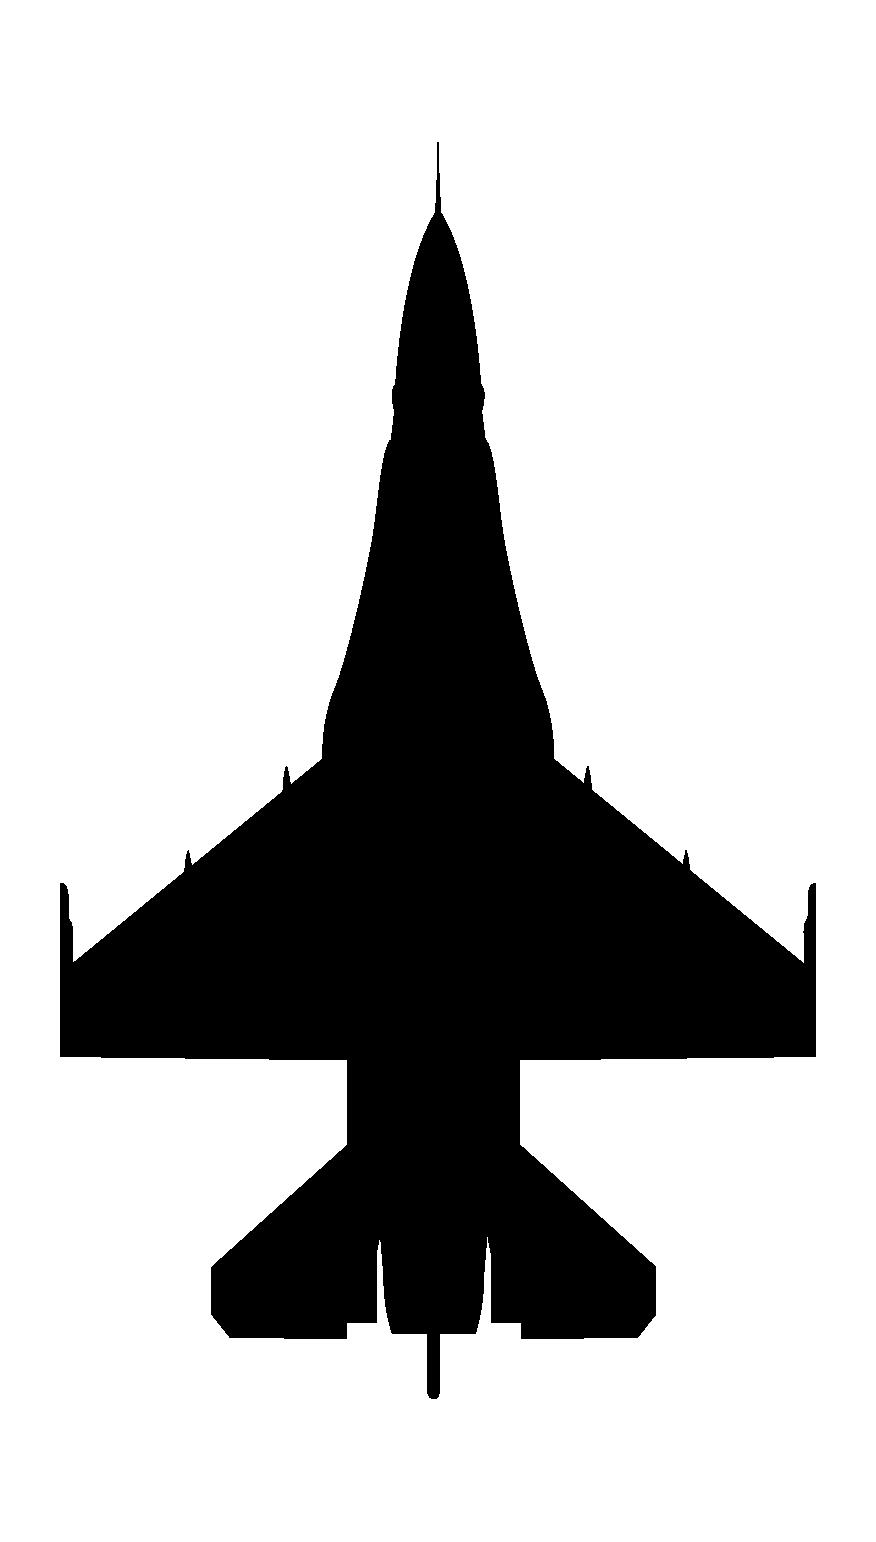
\includegraphics[
                width=7.5mm,
            ]{diagrams/aircraft/silhouette_f16_top.pdf}} 
            ++(0,27.5) 
            arc (0:45:10)  
            -- ++(-5,5) 
            node[above, pos=1, rotate=45]{
                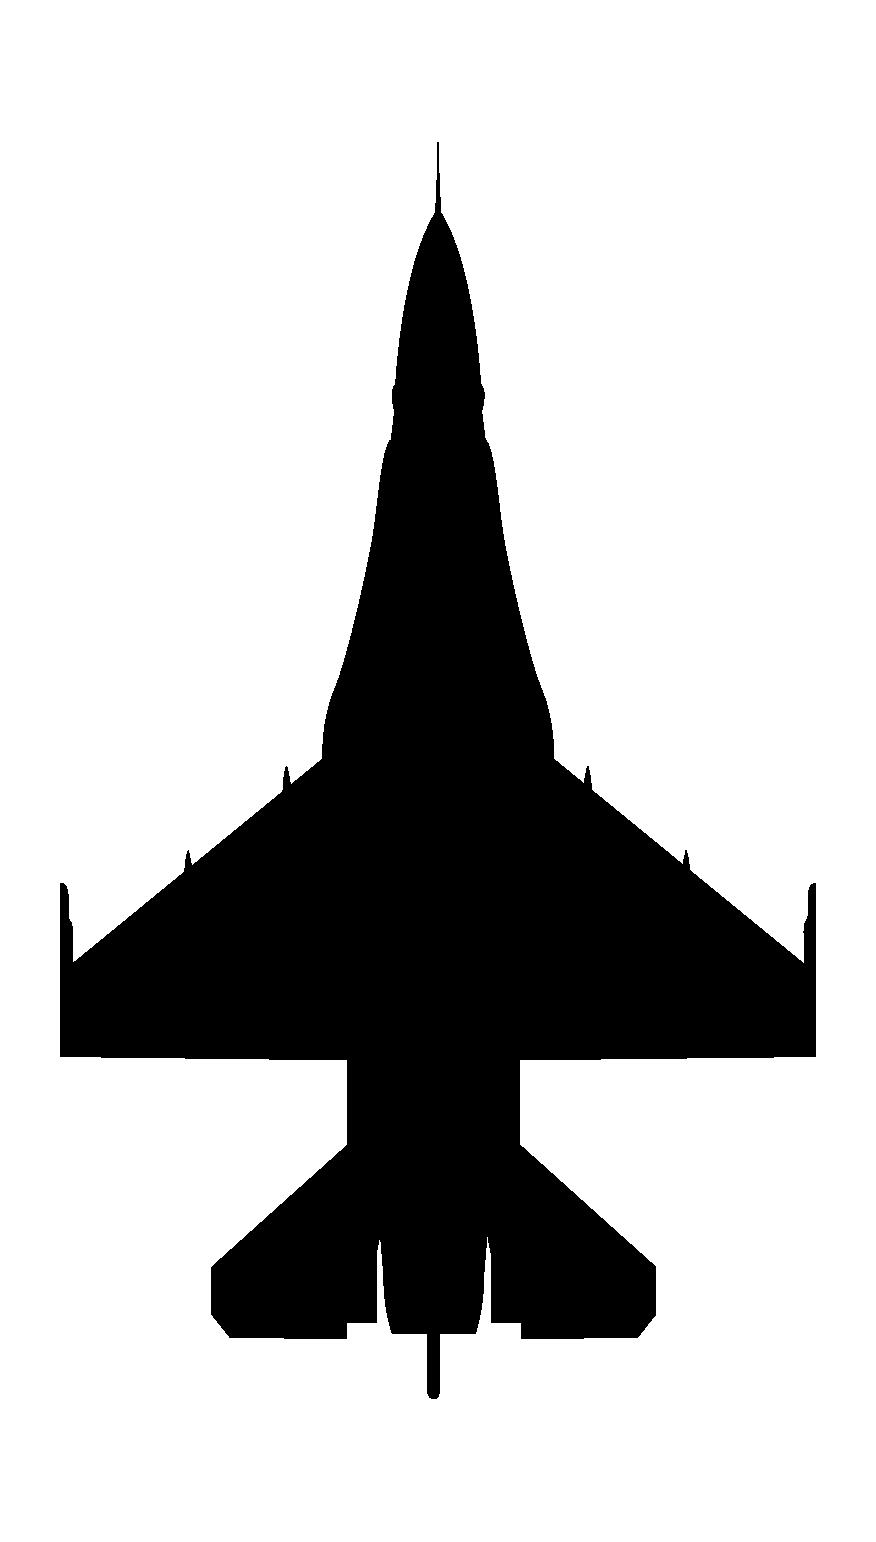
\includegraphics[
                    width=7.5mm,
            ]{diagrams/aircraft/silhouette_f16_top.pdf}};
                
            \draw[->] 
            (10,0) -- 
            node[below, pos=0]{
                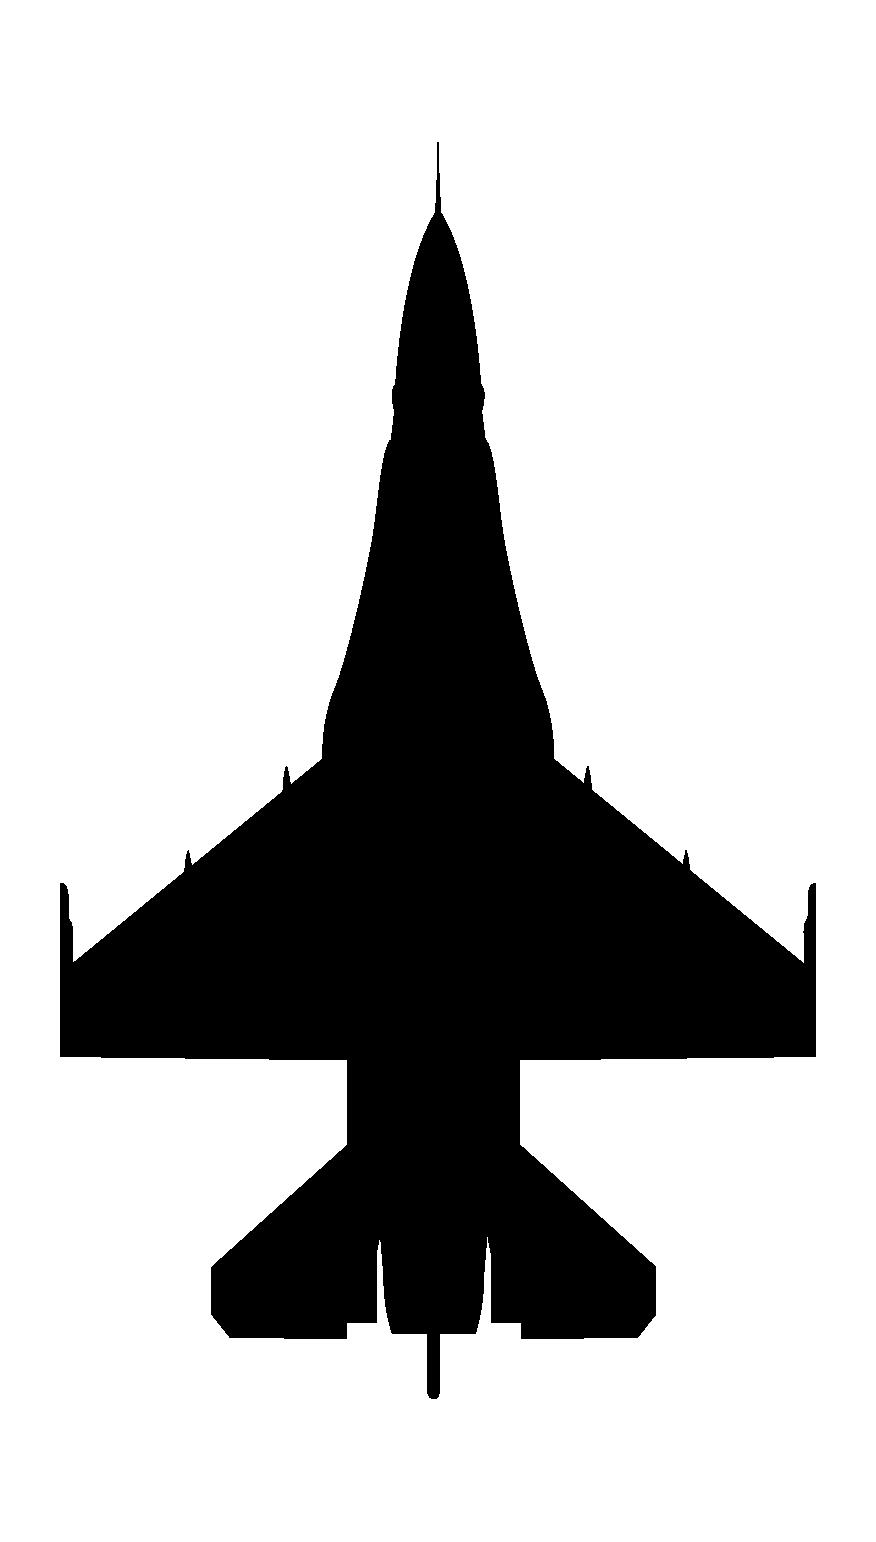
\includegraphics[
                width=7.5mm,
            ]{diagrams/aircraft/silhouette_f16_top.pdf}} 
            ++(0,2.5) 
            arc (0:45:10) 
            -- ++(-22.5,22.5) 
            node[above, pos=1, rotate=45]{
                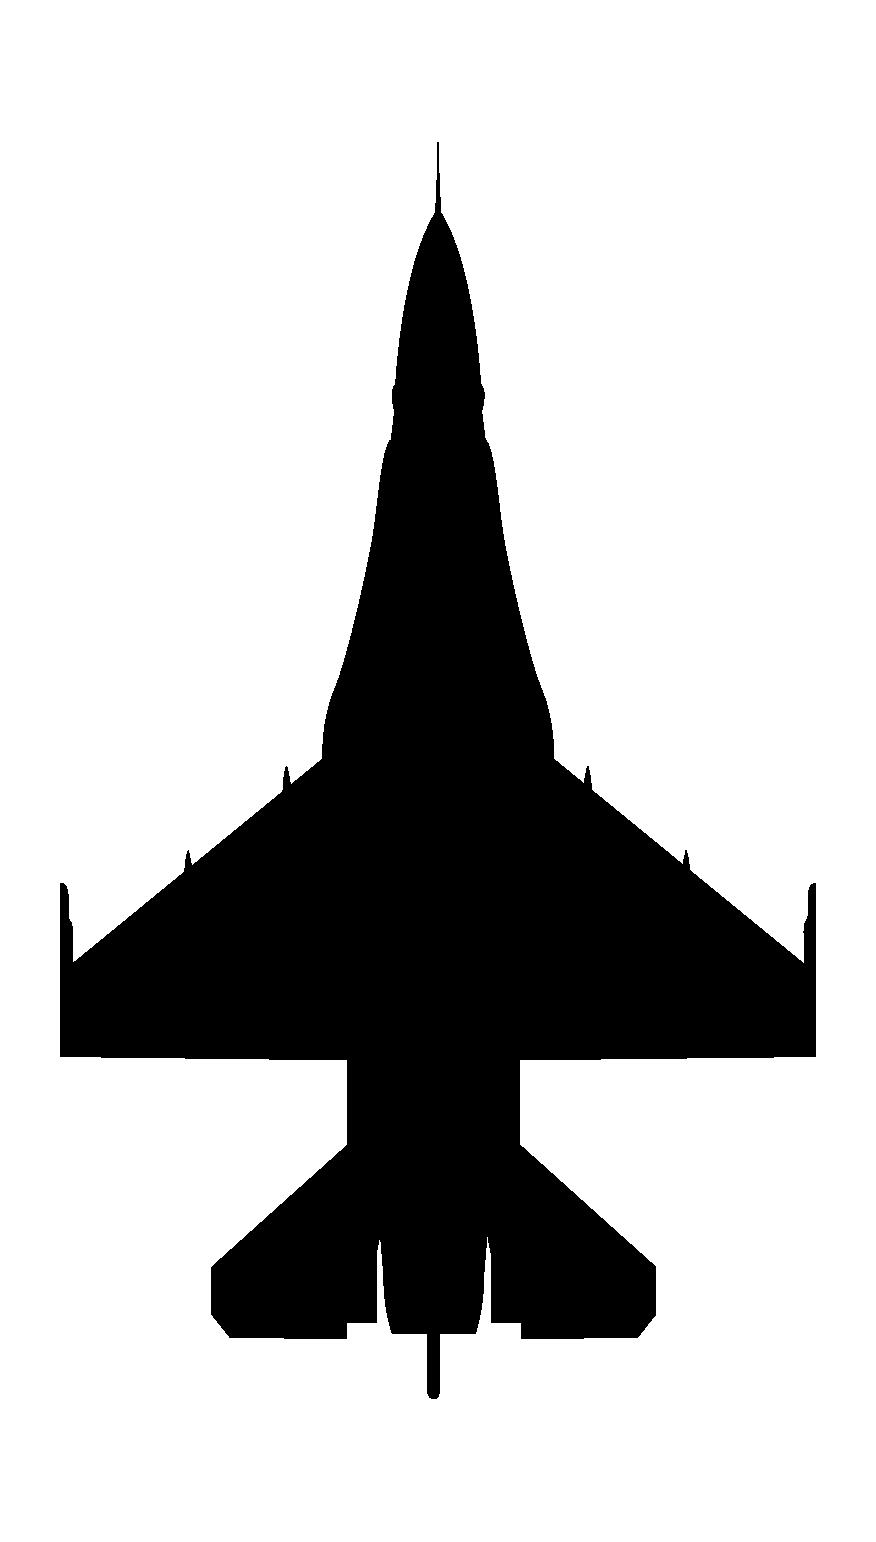
\includegraphics[
                    width=7.5mm,
            ]{diagrams/aircraft/silhouette_f16_top.pdf}};
    
        \end{tikzpicture}
        \caption{45 left}
    \end{subfigure}
    \caption{Tactical turn}
    \label{fig:supp_fig:form:tacturn}
\end{figure}

\begin{figure}[htbp]
    \centering
    \begin{minipage}[b]{0.5\textwidth}
        \centering
        \begin{tikzpicture}[figstyle]
            
            \draw[->] 
            (0,0) -- 
            node[below, pos=0]{
                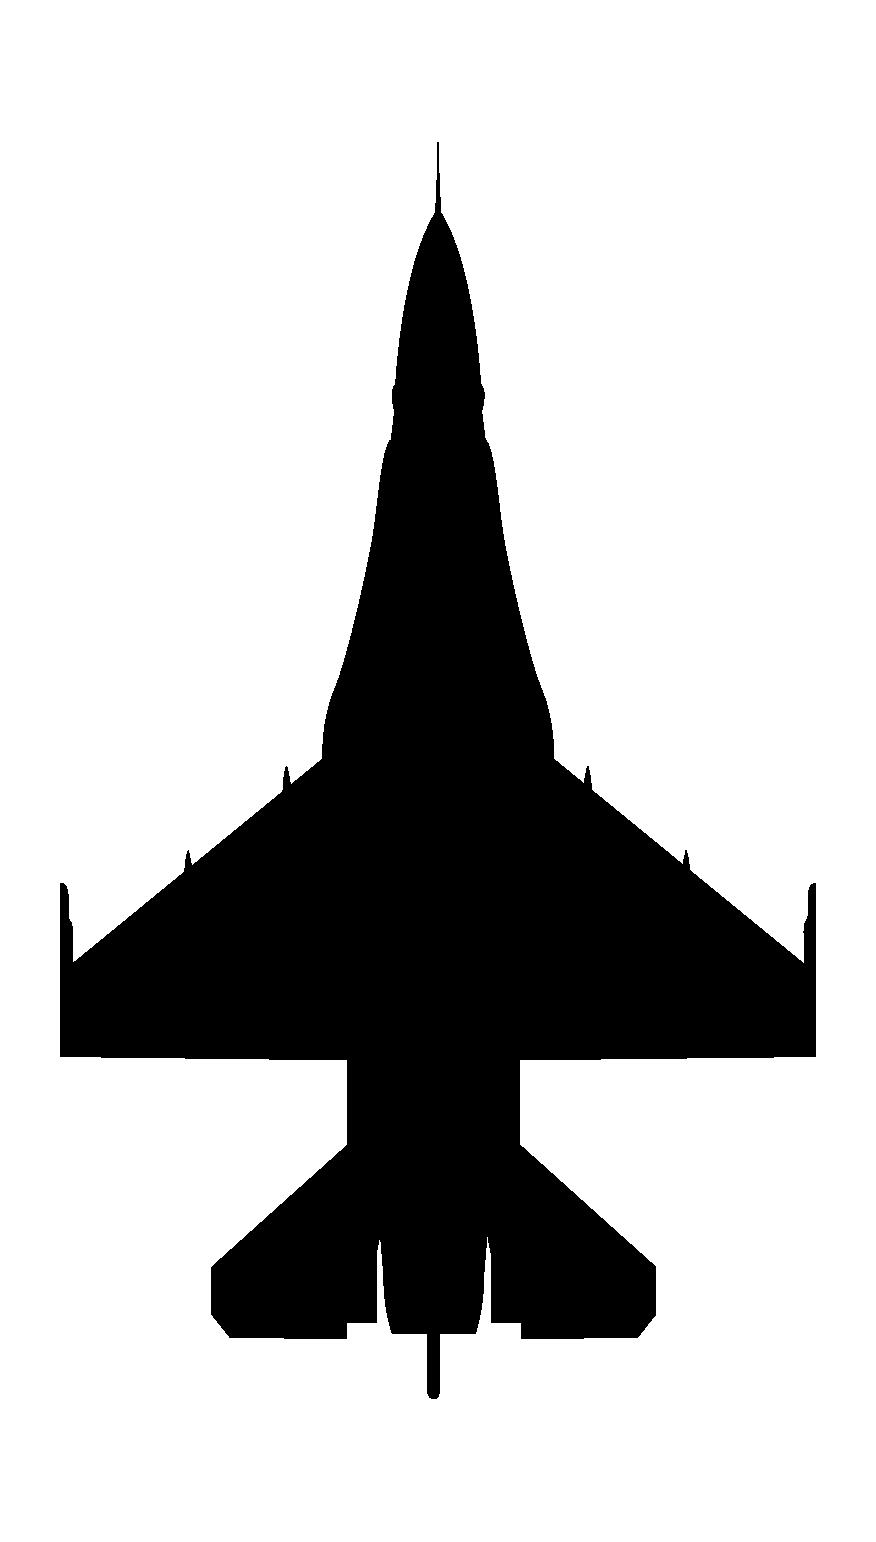
\includegraphics[
                width=7.5mm,
            ]{diagrams/aircraft/silhouette_f16_top.pdf}} 
            ++(0,20) 
            arc (180:00:10) 
            -- ++(0,-10)
            node[above, pos=1, rotate=180]{
                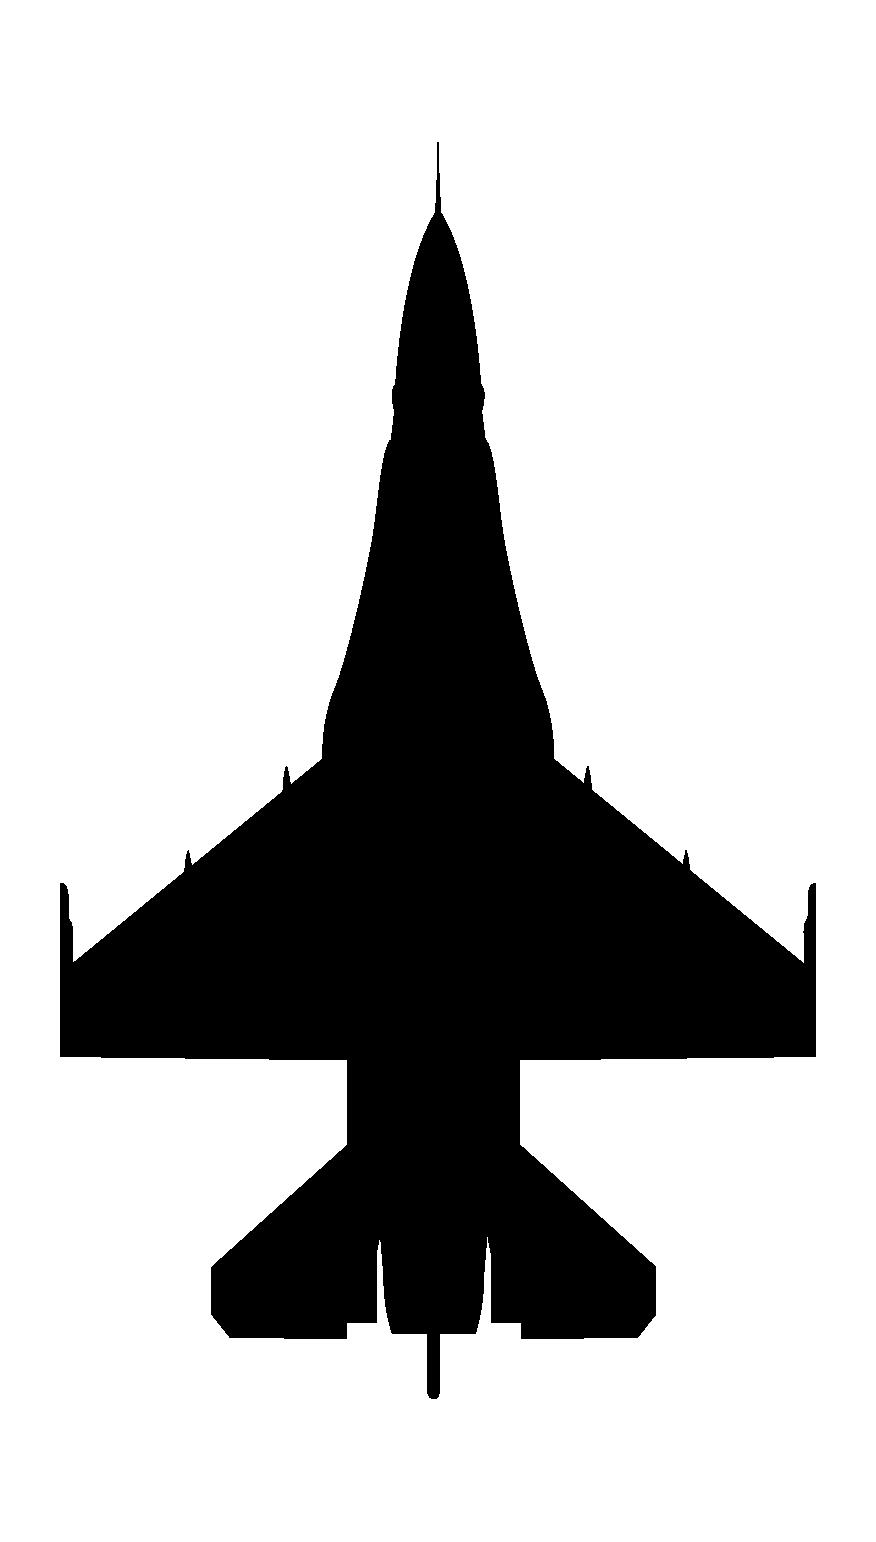
\includegraphics[
                    width=7.5mm,
            ]{diagrams/aircraft/silhouette_f16_top.pdf}};
                
            \draw[->] 
            (10,0) -- 
            node[below, pos=0]{
                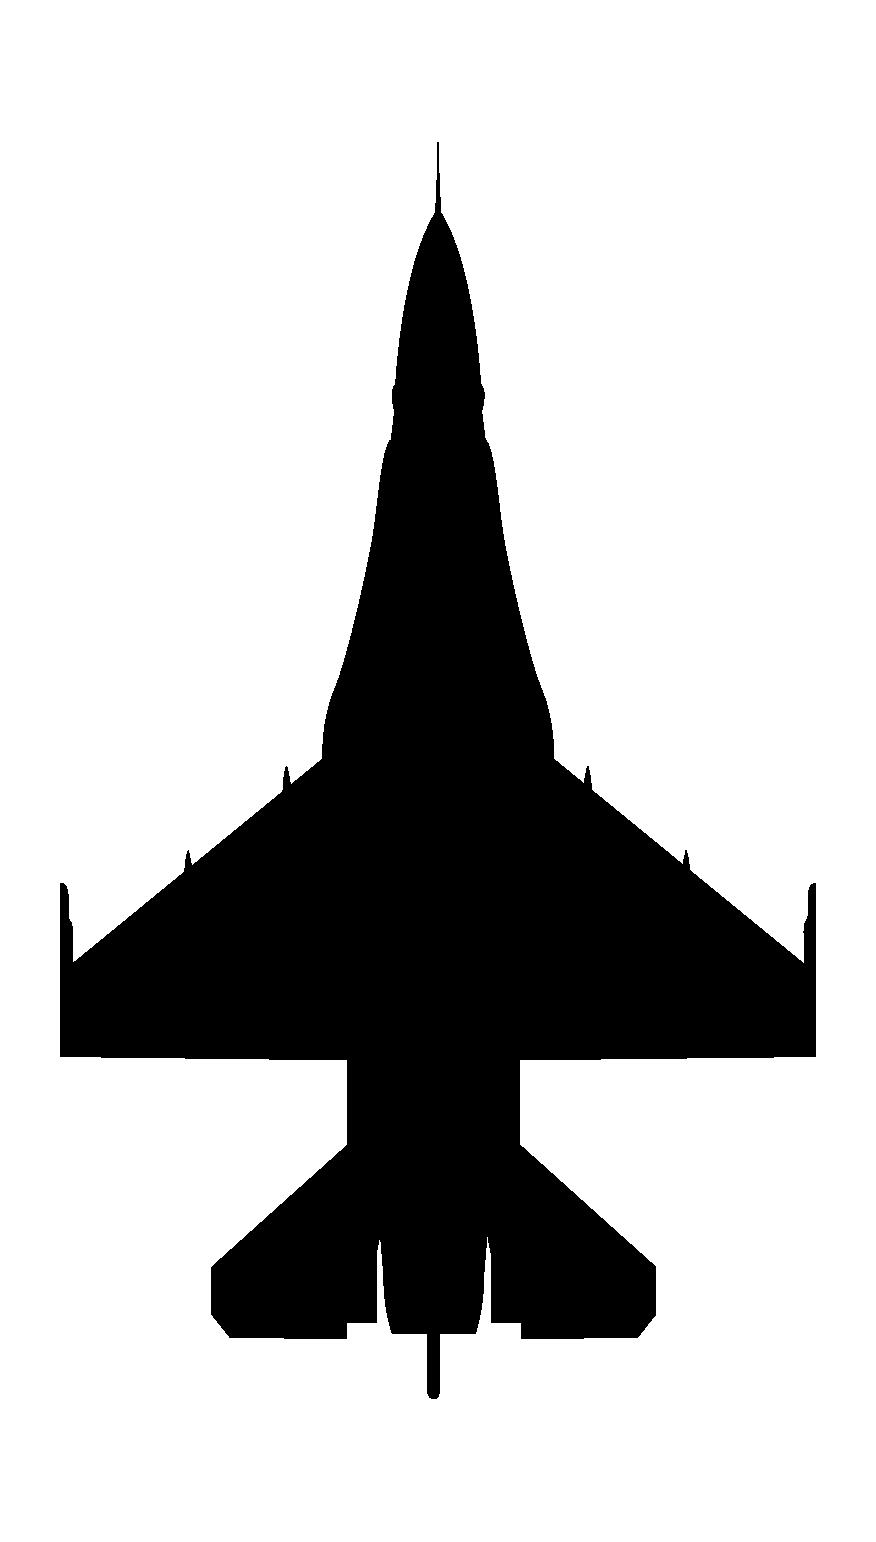
\includegraphics[
                width=7.5mm,
            ]{diagrams/aircraft/silhouette_f16_top.pdf}} 
            ++(0,20) 
            arc (180:0:10) 
            -- ++(0,-10)
            node[above, pos=1, rotate=180]{
                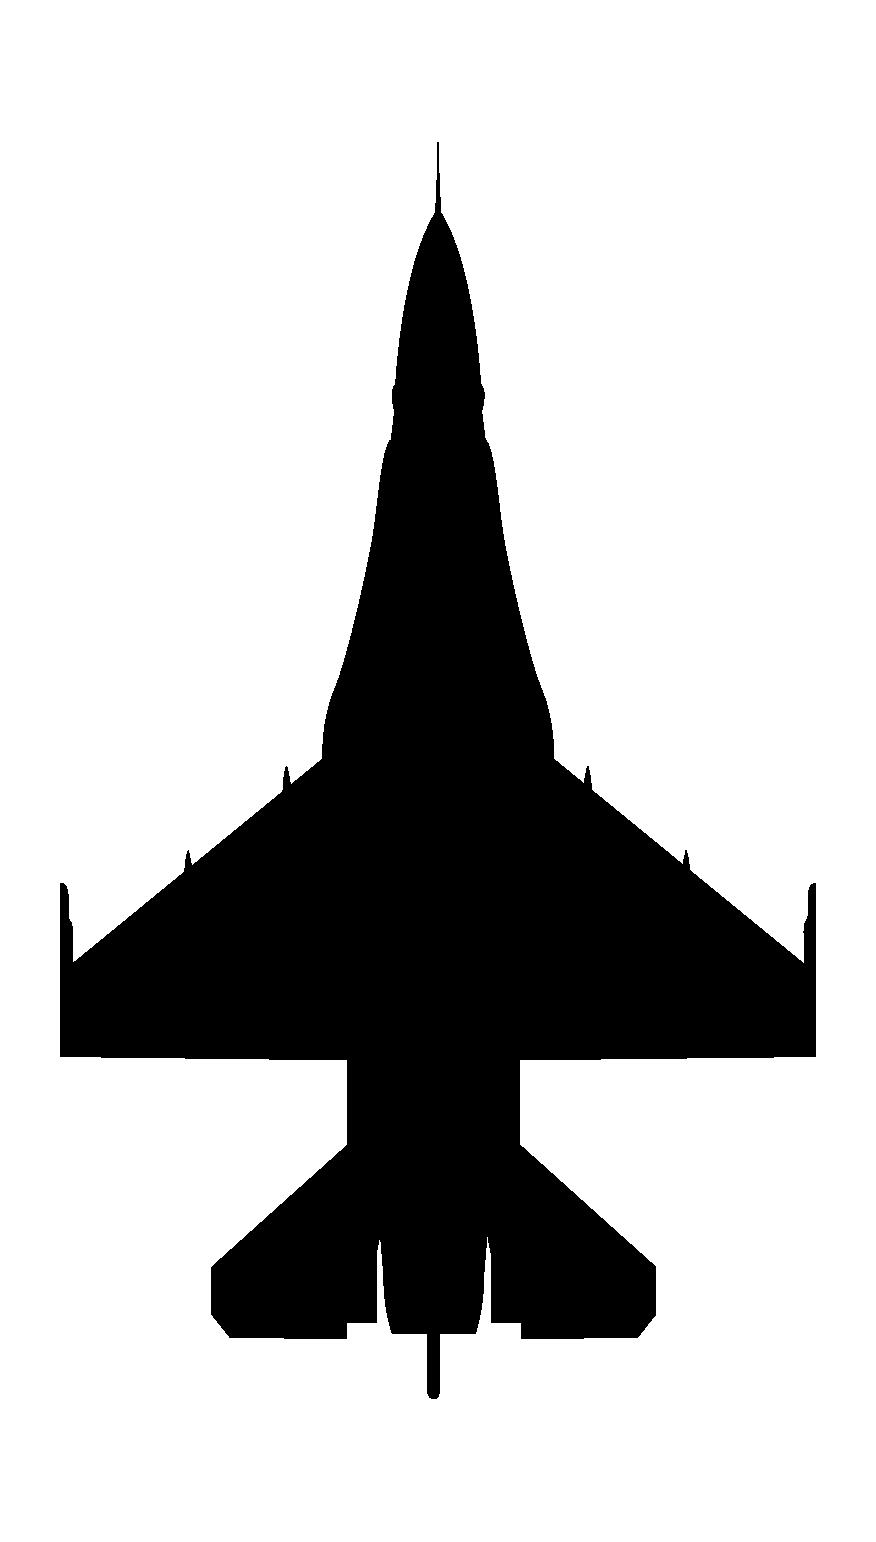
\includegraphics[
                    width=7.5mm,
            ]{diagrams/aircraft/silhouette_f16_top.pdf}};
    
        \end{tikzpicture}
        \caption{Hook turn}
        \label{fig:supp_fig:form:hookturn}
    \end{minipage}%
    \begin{minipage}[b]{0.5\textwidth}
        \centering
        \begin{tikzpicture}[figstyle]
            
            \draw[->] 
            (0,0) -- 
            node[below, pos=0]{
                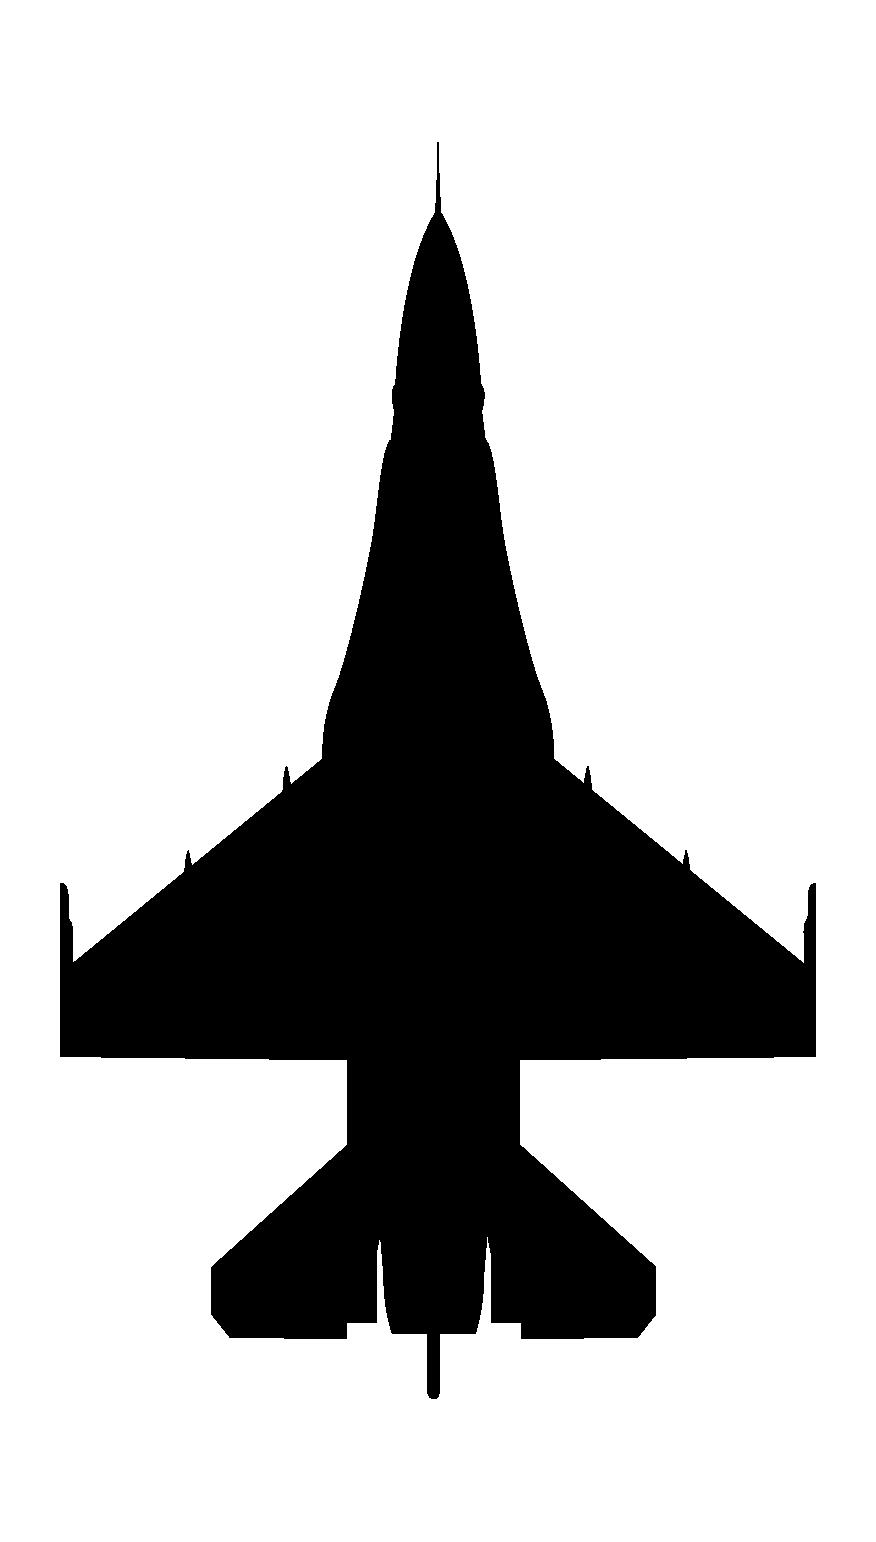
\includegraphics[
                width=7.5mm,
            ]{diagrams/aircraft/silhouette_f16_top.pdf}} 
            ++(0,20) 
            arc (180:00:10) 
            -- ++(0,-10)
            node[above, pos=1, rotate=180]{
                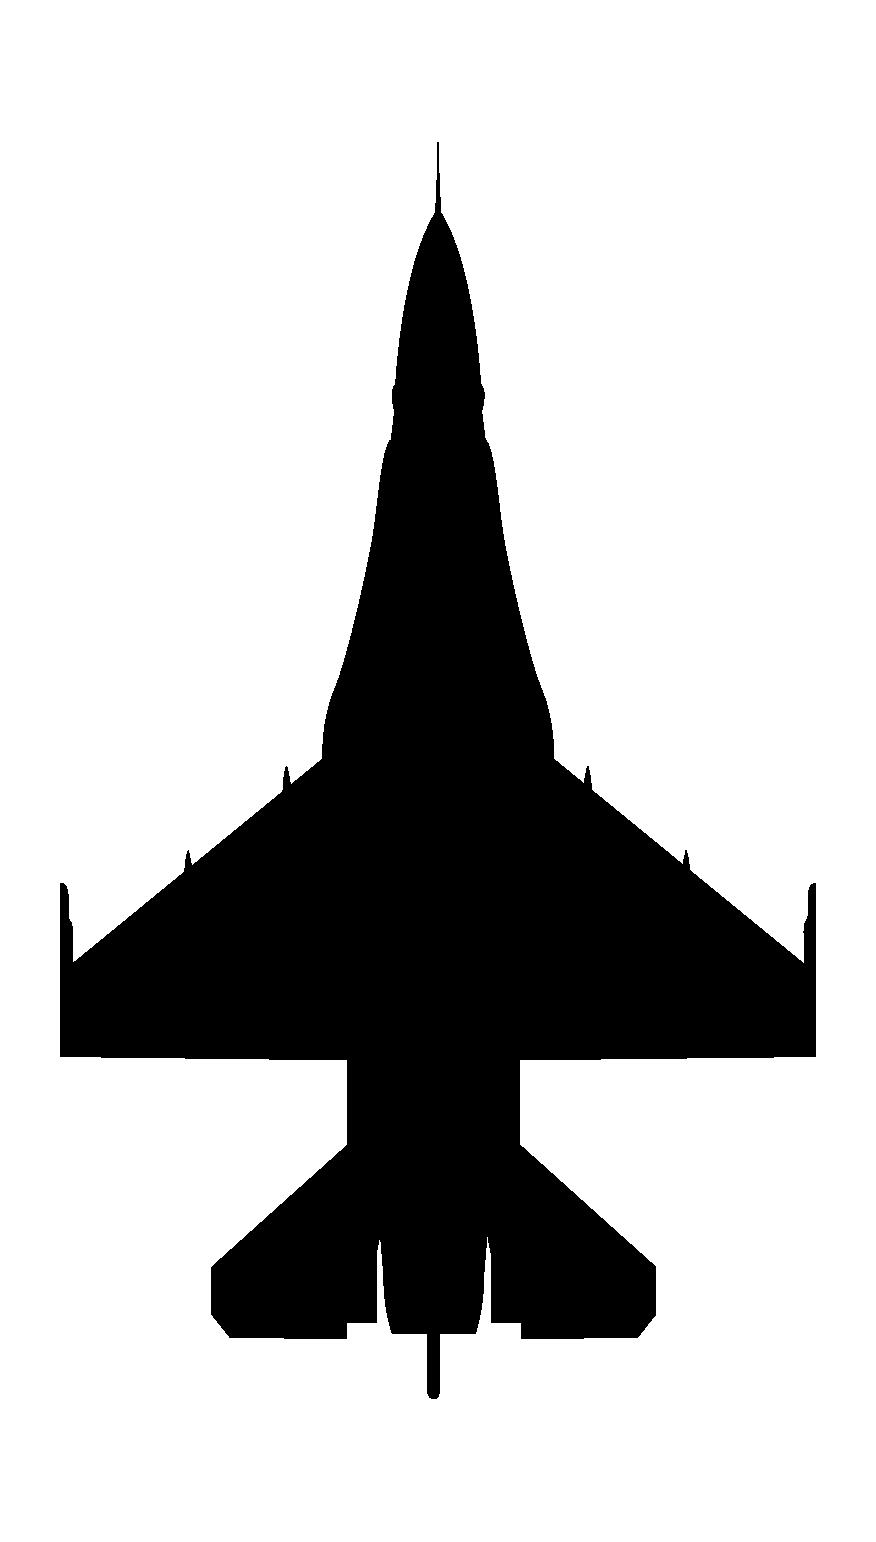
\includegraphics[
                    width=7.5mm,
            ]{diagrams/aircraft/silhouette_f16_top.pdf}};
                
            \draw[->] 
            (10,0) -- 
            node[below, pos=0]{
                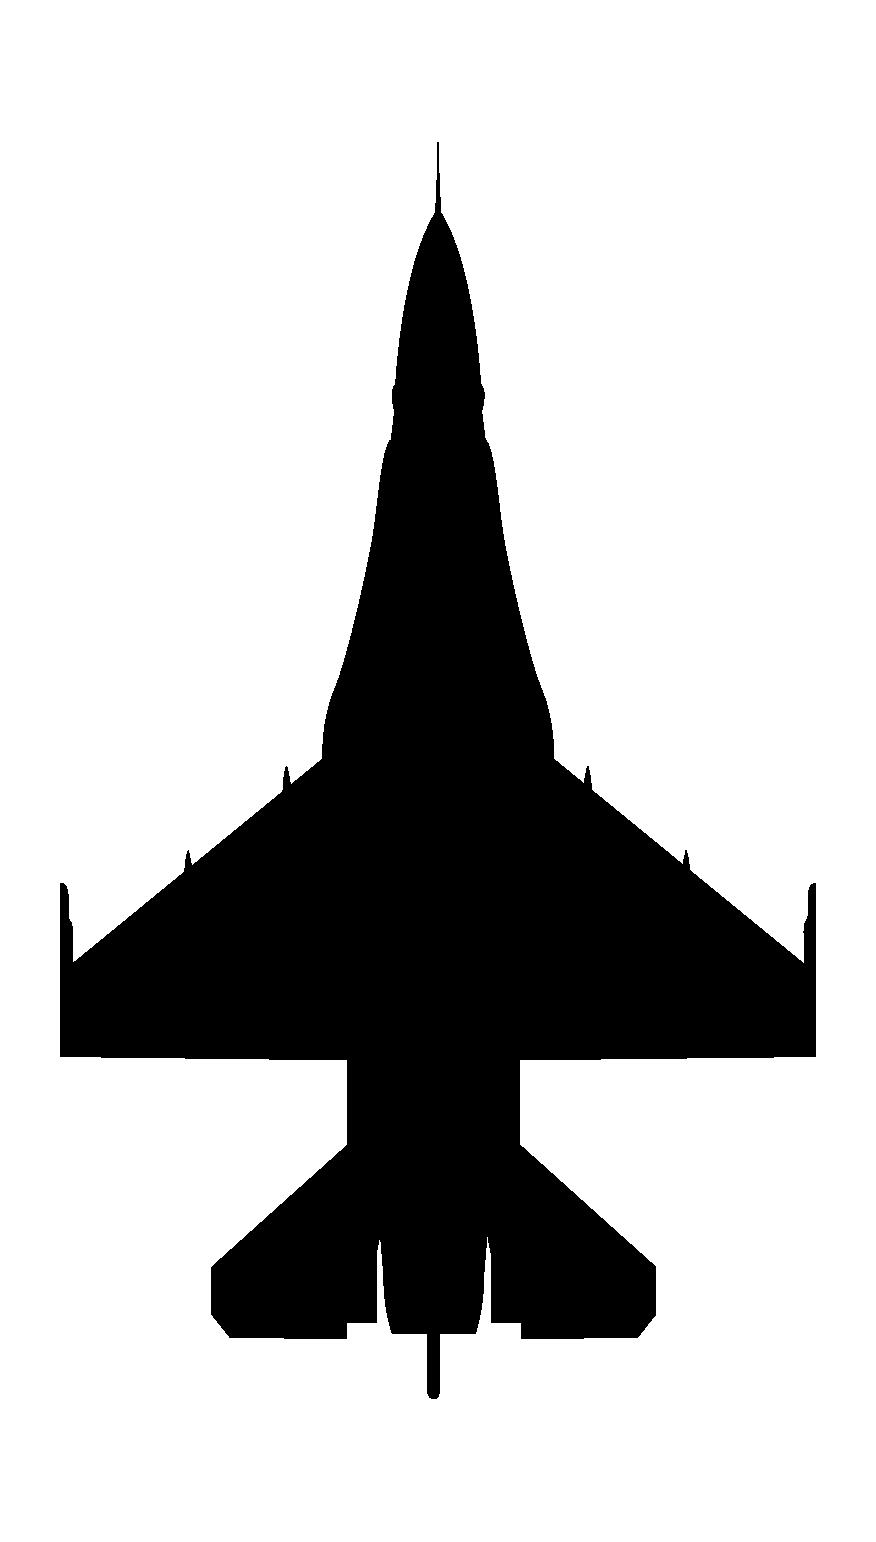
\includegraphics[
                width=7.5mm,
            ]{diagrams/aircraft/silhouette_f16_top.pdf}} 
            ++(0,20) 
            arc (0:180:10) 
            -- ++(0,-10)
            node[above, pos=1, rotate=180]{
                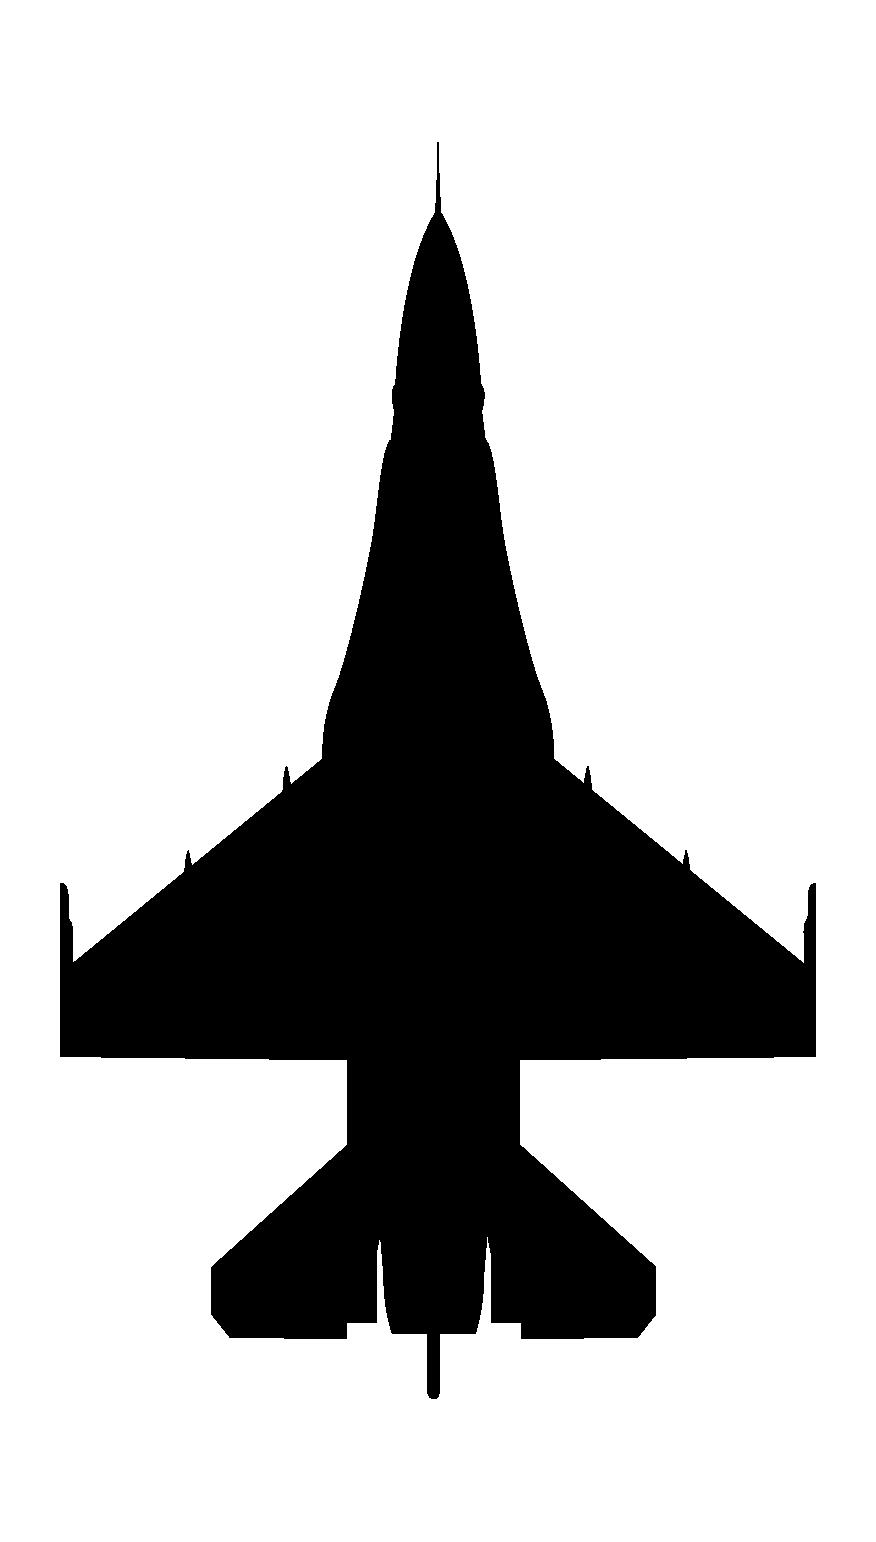
\includegraphics[
                    width=7.5mm,
            ]{diagrams/aircraft/silhouette_f16_top.pdf}};
    
        \end{tikzpicture}
        \caption{Cross turn}
        \label{fig:supp_fig:form:crossturn}
    \end{minipage}
\end{figure}

\begin{figure}[htbp]
    \centering
    \begin{minipage}[b]{0.5\textwidth}
        \centering
        \begin{tikzpicture}[figstyle]
                
            \draw[->] 
            (0,0) -- 
            node[below, pos=0]{
                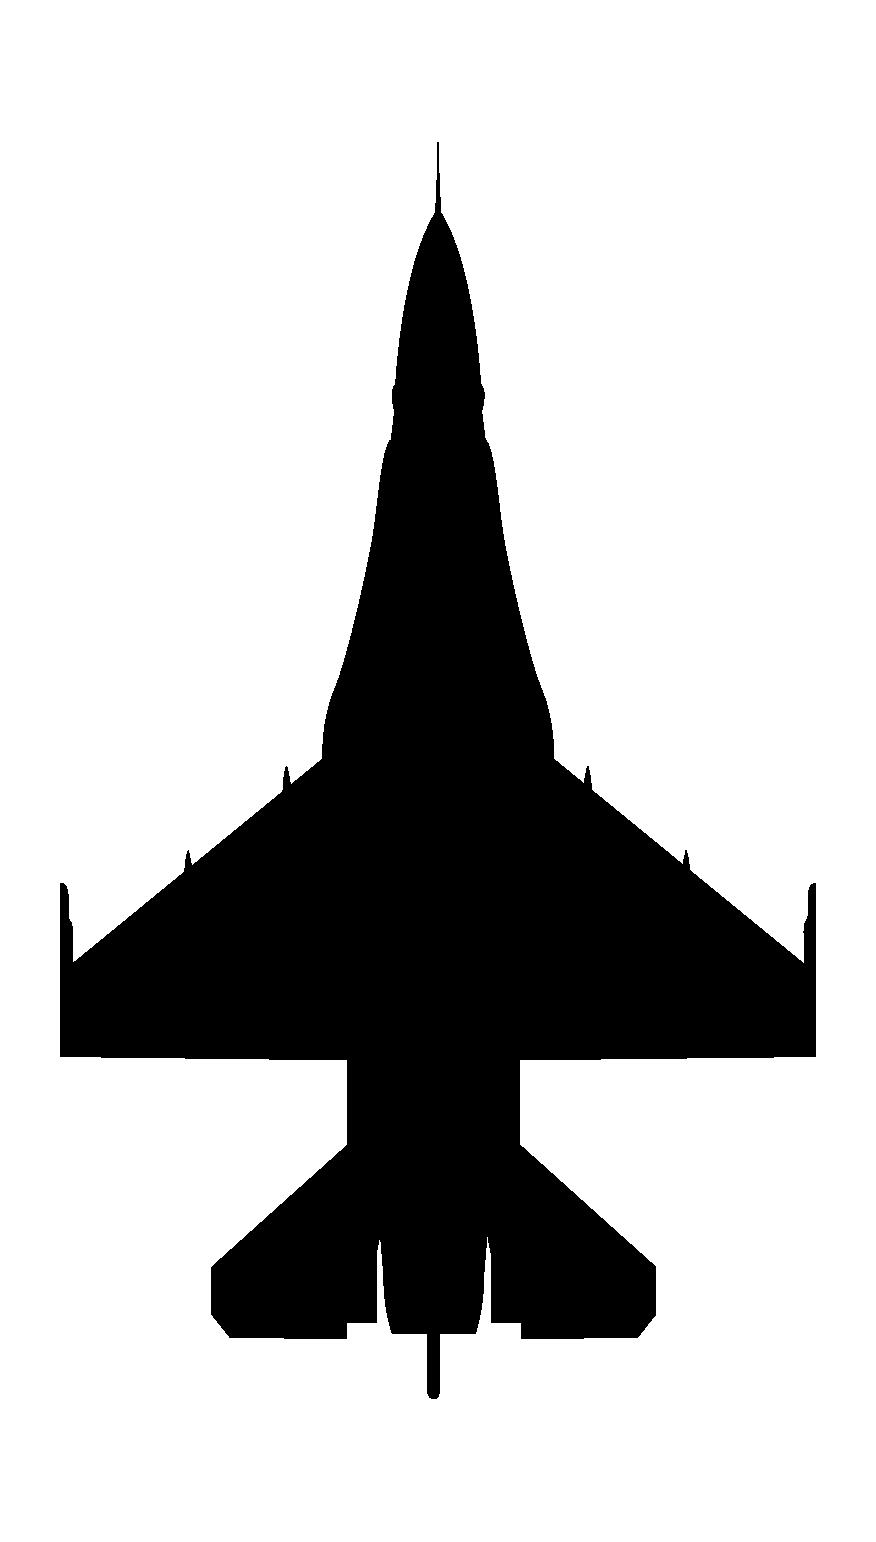
\includegraphics[
                width=7.5mm,
            ]{diagrams/aircraft/silhouette_f16_top.pdf}} 
            ++(0,2.5) 
            arc (180:135:17) 
            arc (-45:0:17) 
            -- ++(0,2.5)
            node[above, pos=1]{
                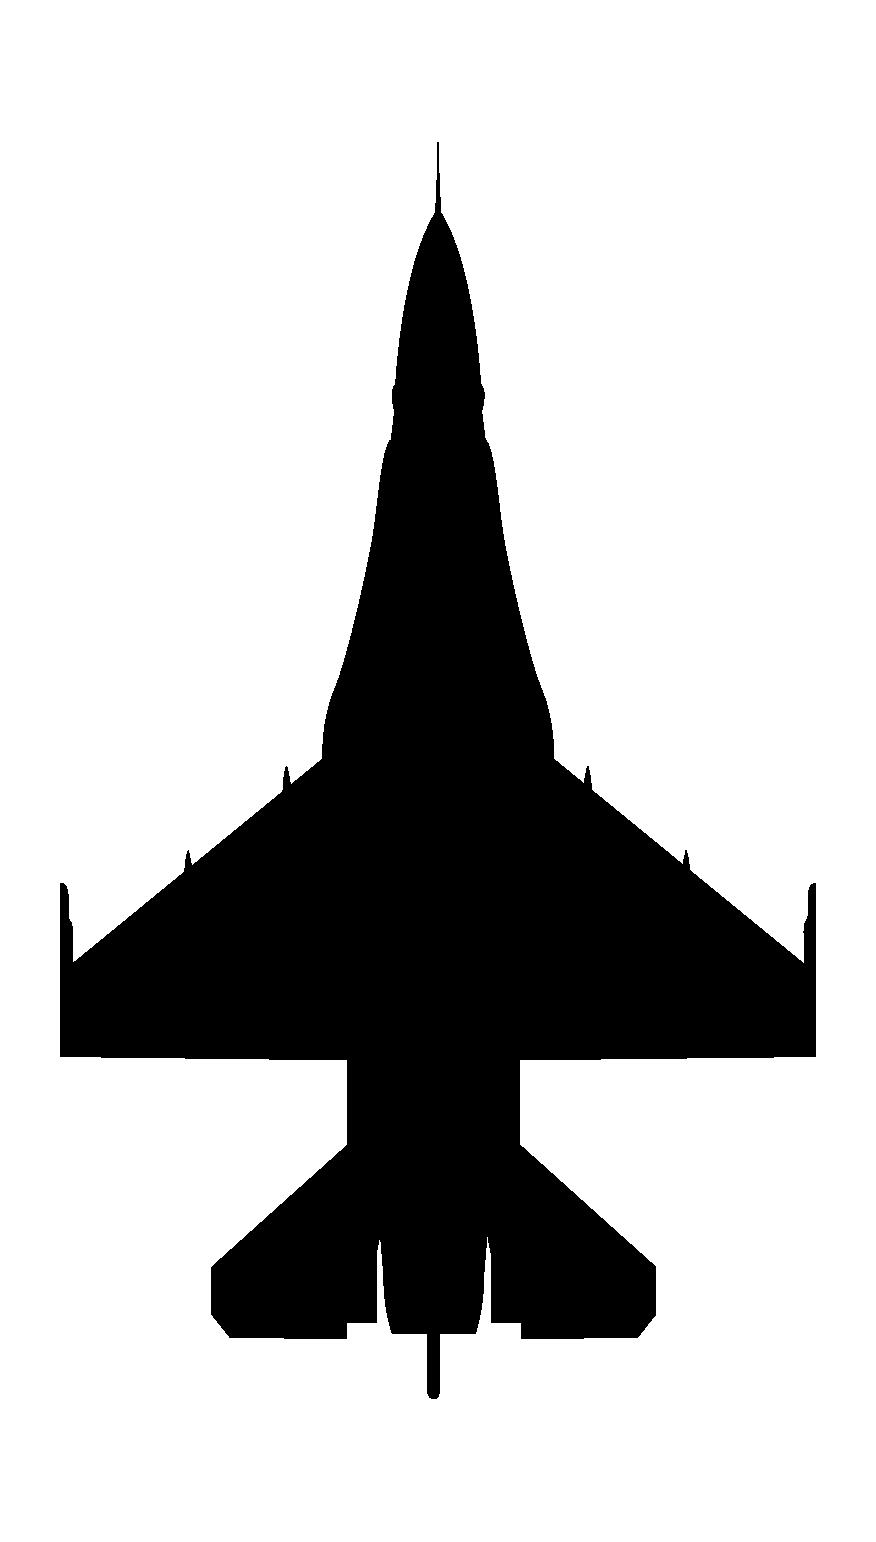
\includegraphics[
                    width=7.5mm,
            ]{diagrams/aircraft/silhouette_f16_top.pdf}};
                
            \draw[->] 
            (10,0) -- 
            node[below, pos=0]{
                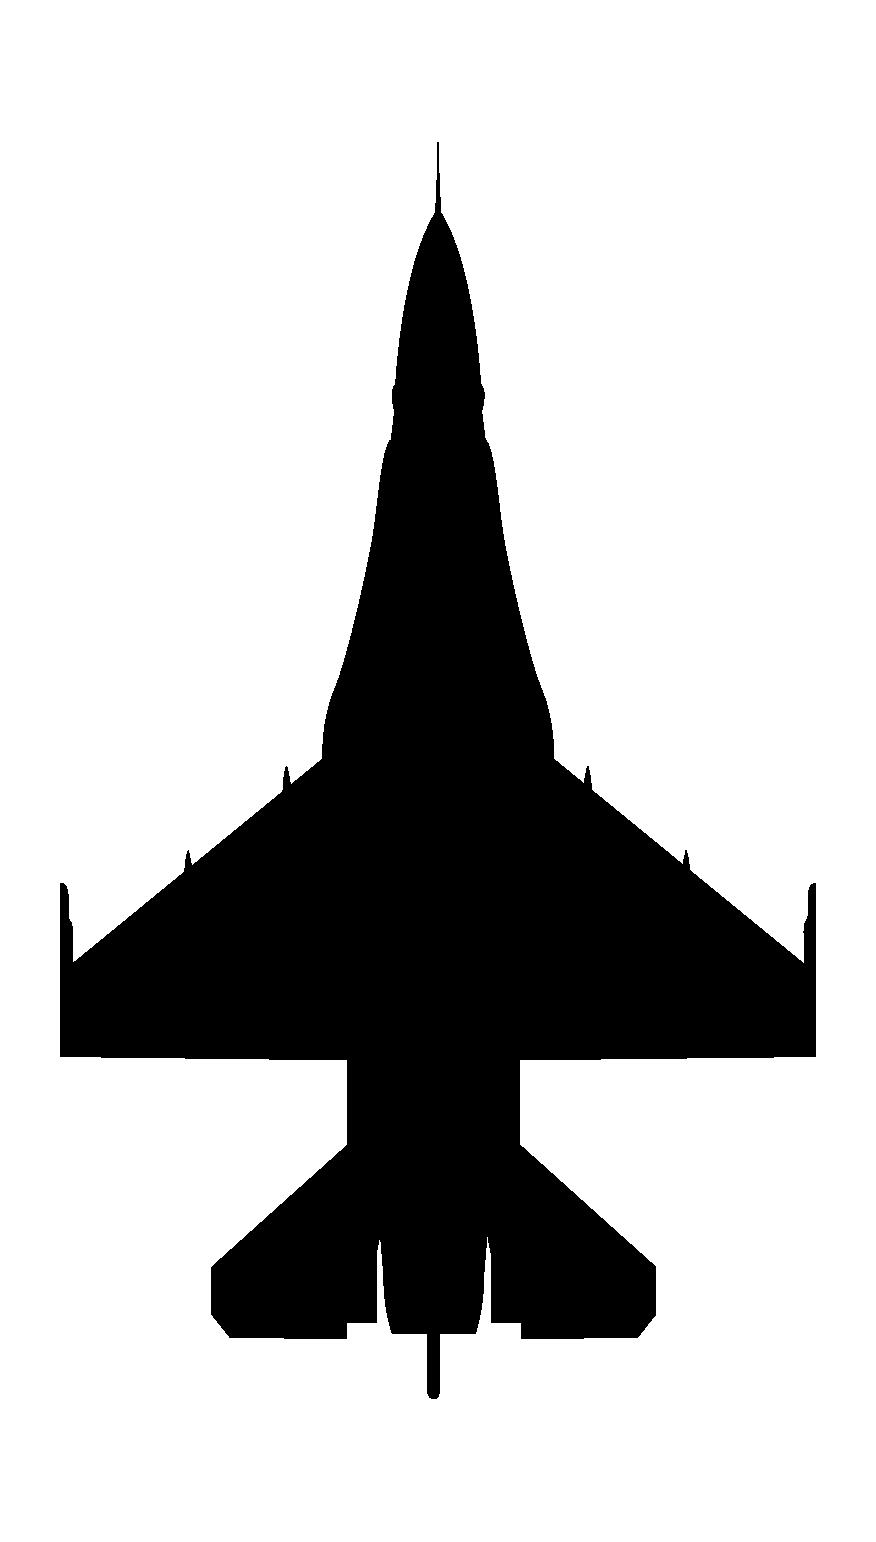
\includegraphics[
                width=7.5mm,
            ]{diagrams/aircraft/silhouette_f16_top.pdf}} 
            ++(0,2.5) 
            arc (0:45:17) 
            arc (-135:-180:17) 
            -- ++(0,2.5)
            node[above, pos=1]{
                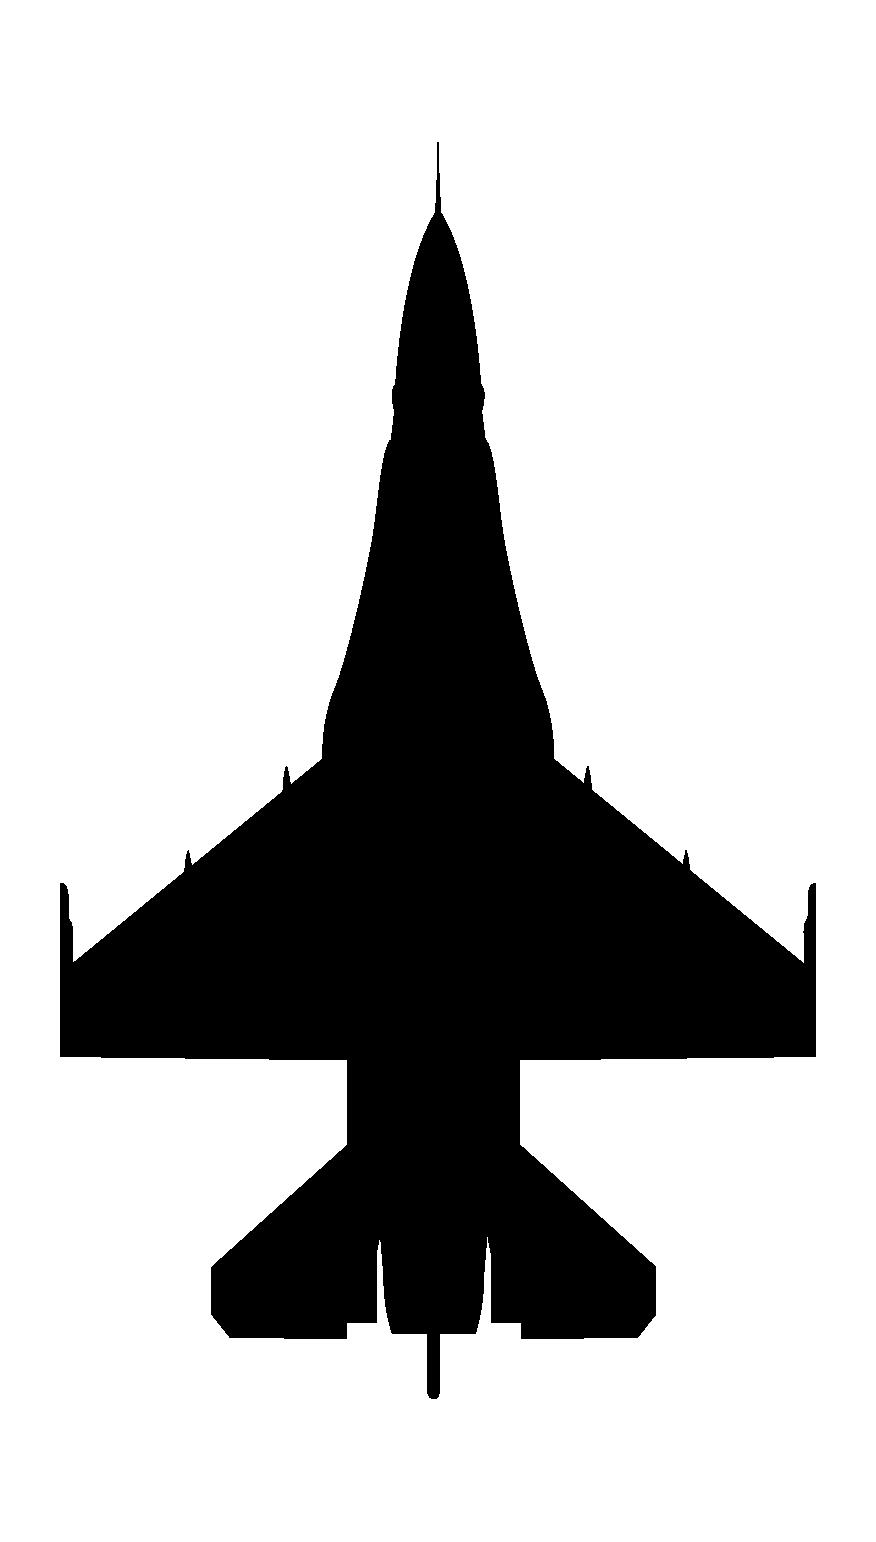
\includegraphics[
                    width=7.5mm,
            ]{diagrams/aircraft/silhouette_f16_top.pdf}};

        \end{tikzpicture}
        \caption{Shackle}
        \label{fig:supp_fig:form:shackle}
    \end{minipage}%
    \begin{minipage}[b]{0.5\textwidth}
        \centering
        \begin{tikzpicture}[figstyle]
            
            \draw[->] 
            (0,0) -- 
            node[below, pos=0]{
                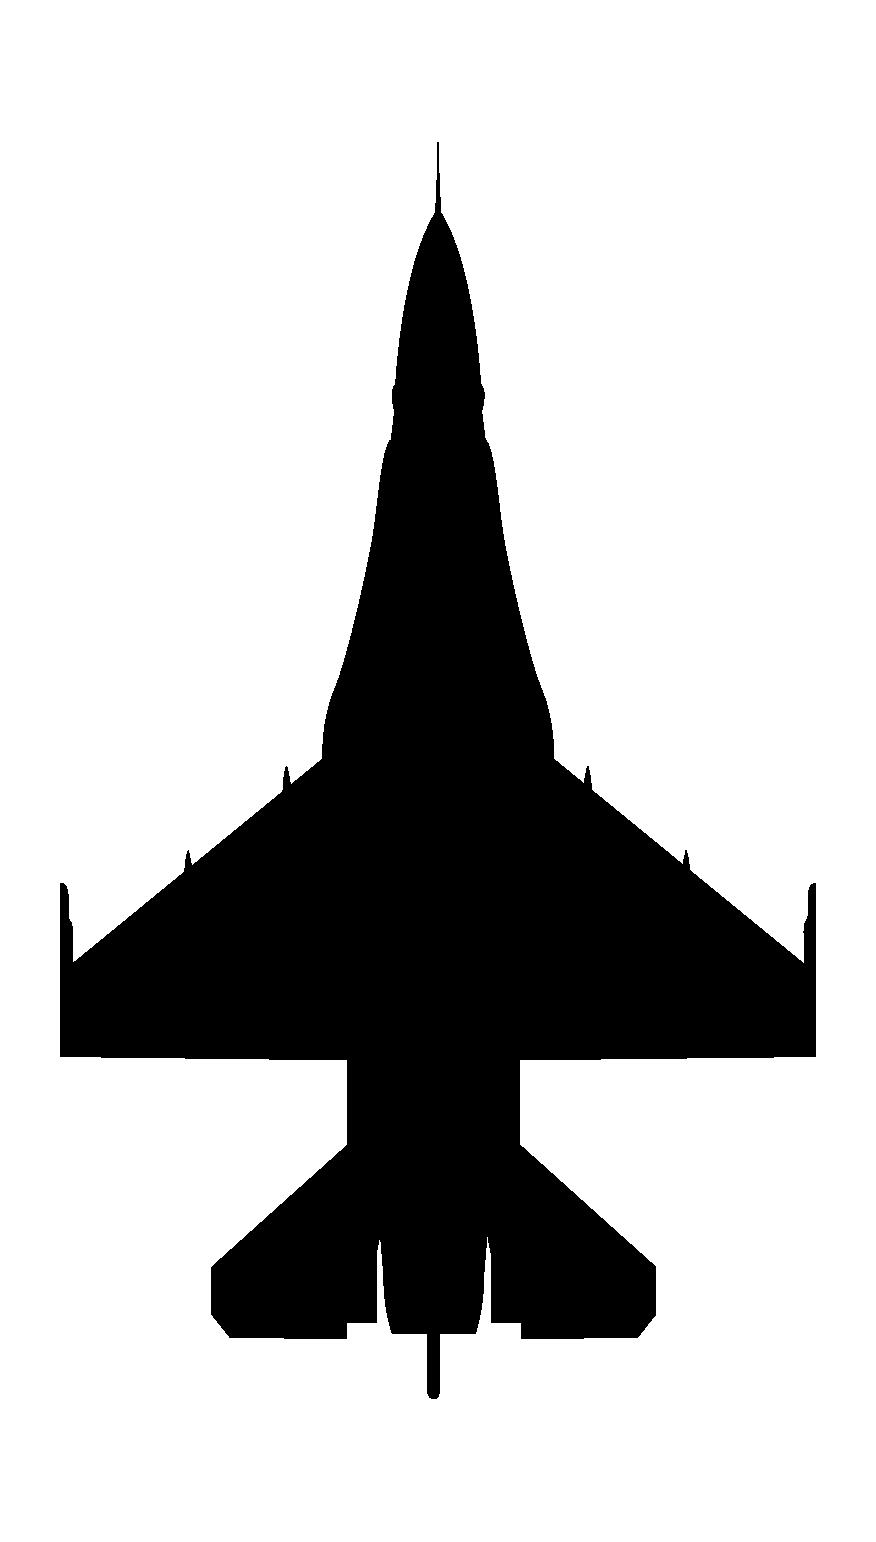
\includegraphics[
                width=7.5mm,
            ]{diagrams/aircraft/silhouette_f16_top.pdf}} 
            ++(0,10) 
            arc (180:90:10) 
            % -- ++(0,0)
            node[above, pos=1, rotate=-90]{
                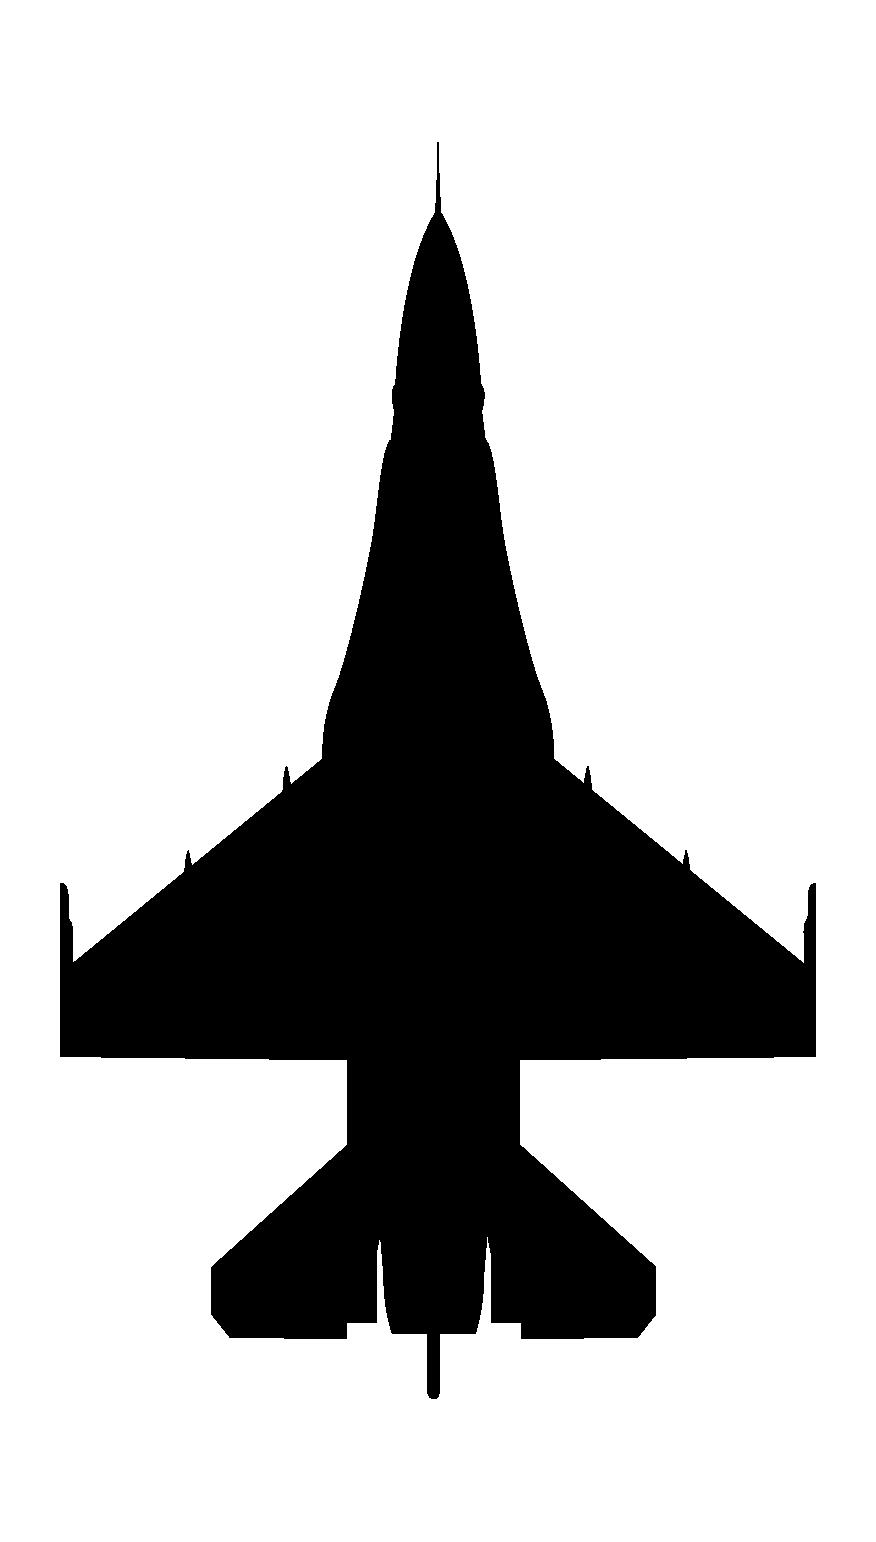
\includegraphics[
                    width=7.5mm,
            ]{diagrams/aircraft/silhouette_f16_top.pdf}};
                
            \draw[->] 
            (20,0) -- 
            node[below, pos=0]{
                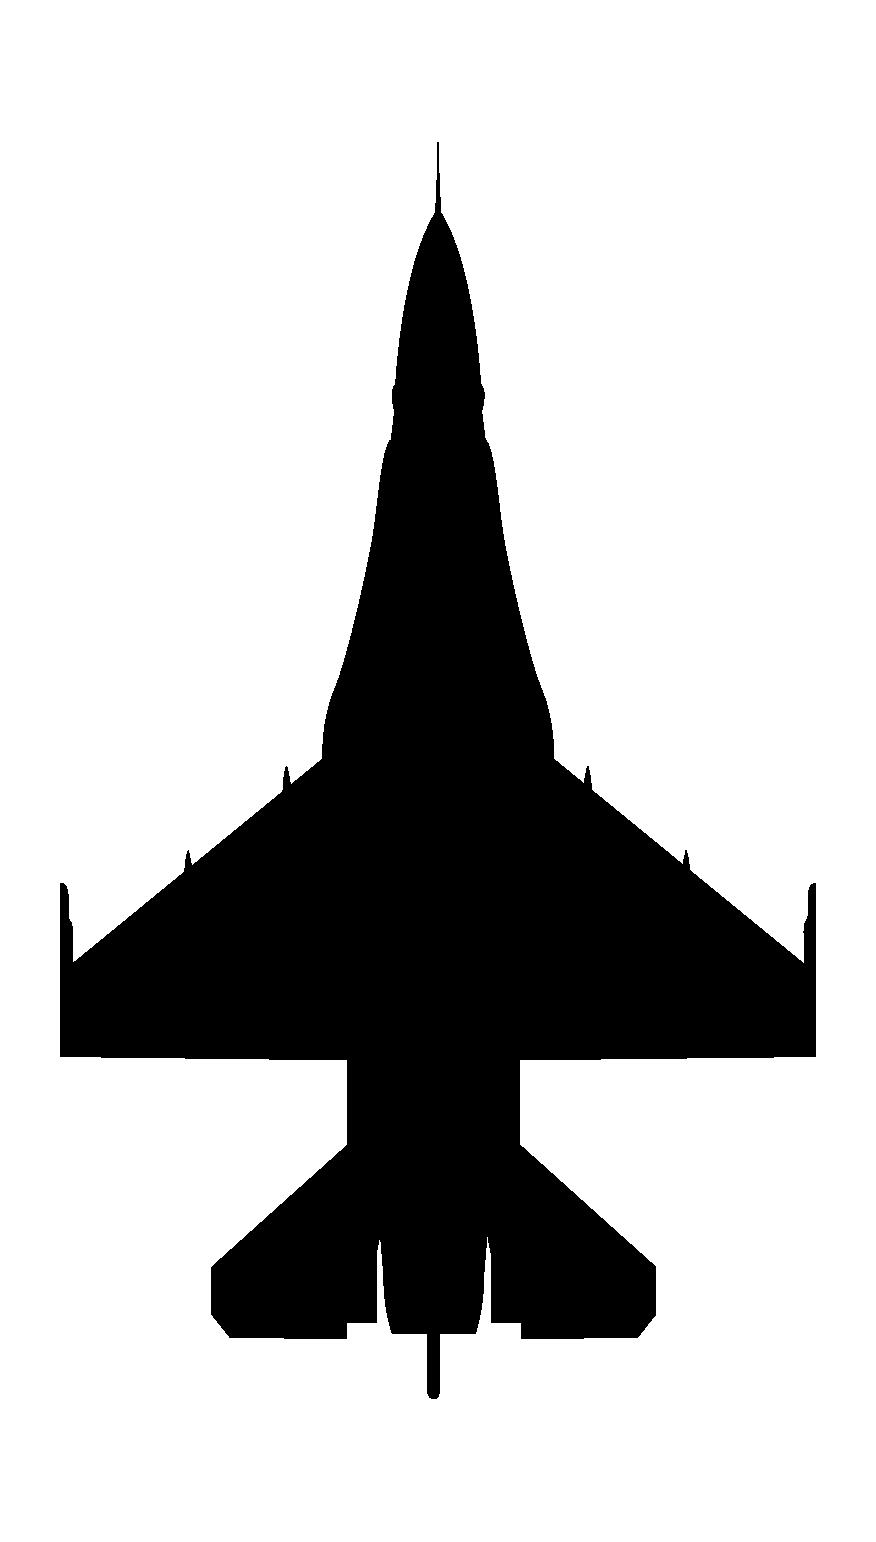
\includegraphics[
                width=7.5mm,
            ]{diagrams/aircraft/silhouette_f16_top.pdf}} 
            ++(0,10) 
            arc (180:90:10) 
            % -- ++(0,0)
            node[above, pos=1, rotate=-90]{
                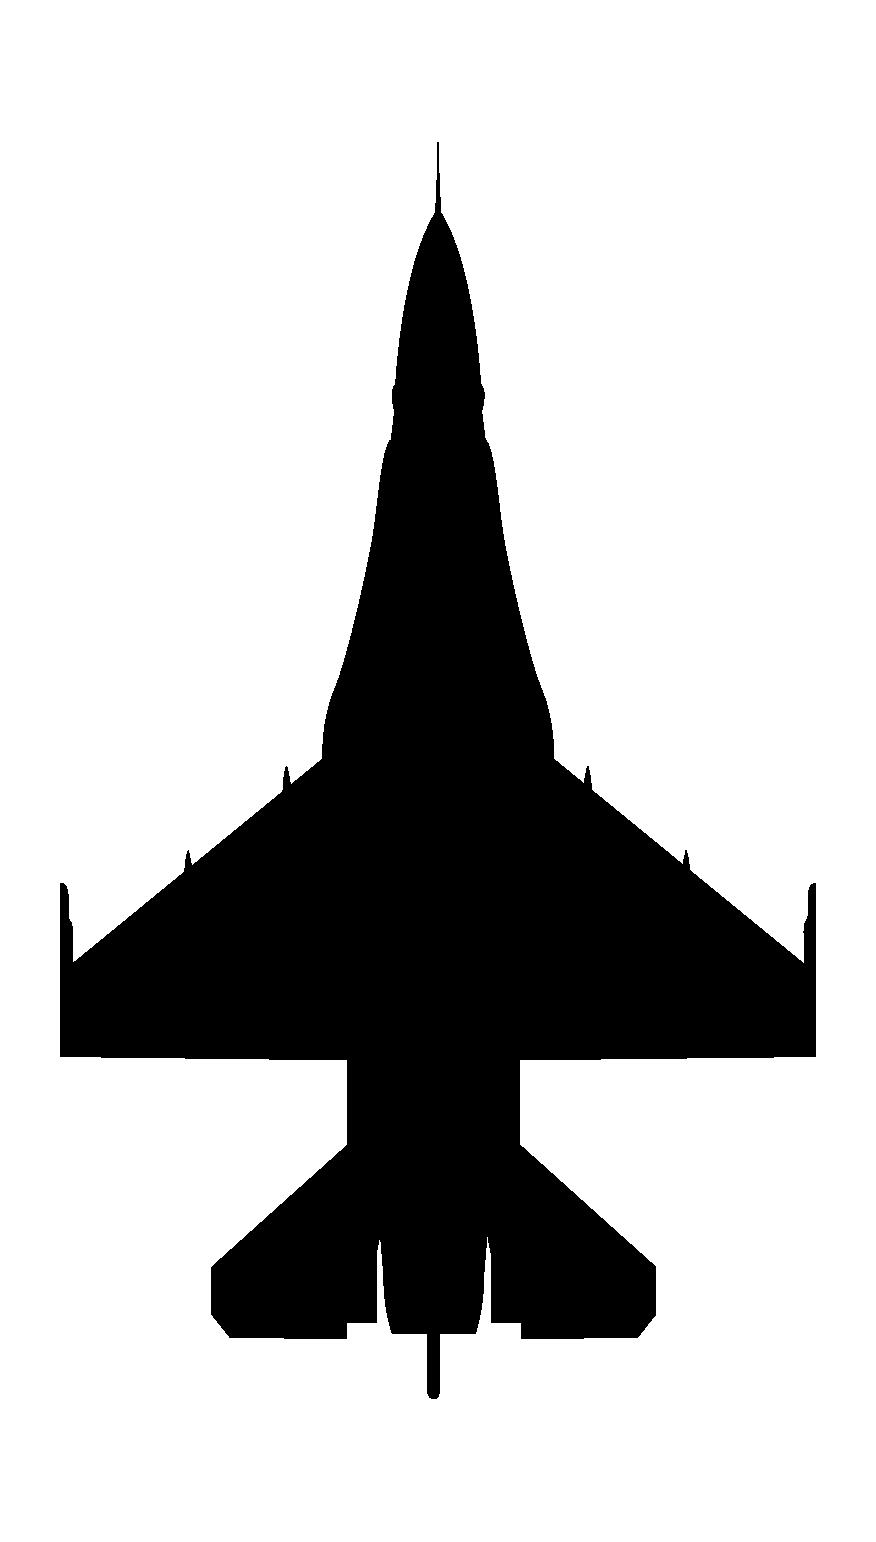
\includegraphics[
                    width=7.5mm,
            ]{diagrams/aircraft/silhouette_f16_top.pdf}};
    
        \end{tikzpicture}
        \caption{In-place 90 right}
        \label{fig:supp_fig:form:inplace}
    \end{minipage}
\end{figure}

\notebox{
    \small Wingman is responsible for deconfliction during maneuvers. Do \textbf{NOT} hit lead!
}
\begin{tcoloritemize}
    \blueitem[Overhead \break Approach]
    Reference \cref{subsec:proc_basic:to_ldg:ldg} for landing procedure.
    \begin{itemize}
        \item flight should be in echelon right/left
        \item lead breaks first, 2-4 in 5 second intervals 
    \end{itemize}
    \hfill\textbf{Reference \cref{fig:supp_fig:form:overhead}}
\end{tcoloritemize}

\begin{figure}[htbp]
    \centering
    \begin{tikzpicture}[figstyle]

        % coordinates
        \coordinate (approach1) at (5,-25);
        \coordinate (approach2) at (10,-30);
        \coordinate (approach3) at (15,-35);
        \coordinate (approach4) at (20,-40);
        \coordinate (break1) at (5,20);
        \coordinate (break2) at (10,25);
        \coordinate (break3) at (15,30);
        \coordinate (break4) at (20,35);
        \coordinate (downwind) at (-15,20);
        \coordinate (base) at (-15,-15);
        \coordinate (final) at (-7.5,-22.5);
        \coordinate (shortfinal) at (0,-15);
        \coordinate (touchdown) at (0,0);
        \coordinate (rollout) at (0,20);

        % runway
        \draw[thick]
        ($(touchdown)+(-2,-5)$) -- ($(touchdown)+(2,-5)$) -- 
        ($(touchdown)+(2,25)$) -- ($(touchdown)+(-2,25)$) -- 
        cycle;
        \draw[thick]
        ($(touchdown)+(-1.33,-1)$) -- ($(touchdown)+(-1.33,1)$)
        ($(touchdown)+(-0.66,-1)$) -- ($(touchdown)+(-0.66,1)$)
        ($(touchdown)+(0.66,-1)$) -- ($(touchdown)+(0.66,1)$)
        ($(touchdown)+(1.33,-1)$) -- ($(touchdown)+(1.33,1)$);

        % pattern
        \draw[ultra thick, ->] 
        (approach1) -- (break1);
        \draw[ultra thick, ->] 
        (approach2) -- (break2);
        \draw[ultra thick, ->] 
        (approach3) -- (break3);
        \draw[ultra thick, ->] 
        (approach4) -- (break4);
        \draw[ultra thick] 
        (break1) arc (0:180:10)
        (break2) arc (0:180:12.5)
        (break3) arc (0:180:15)
        (break4) arc (0:180:17.5) -- (downwind);
        \draw[ultra thick, >->] 
        (downwind) -- (base);
        \draw[ultra thick] 
        (base) arc (180:270:7.5);
        \draw[ultra thick] 
        (final) arc (270:360:7.5);
        \draw[ultra thick, >-] 
        (shortfinal) -- (touchdown);
        \draw[ultra thick, ->] 
        (touchdown) -- (rollout);

        % nodes
        \node[below] at (approach1)
        {
            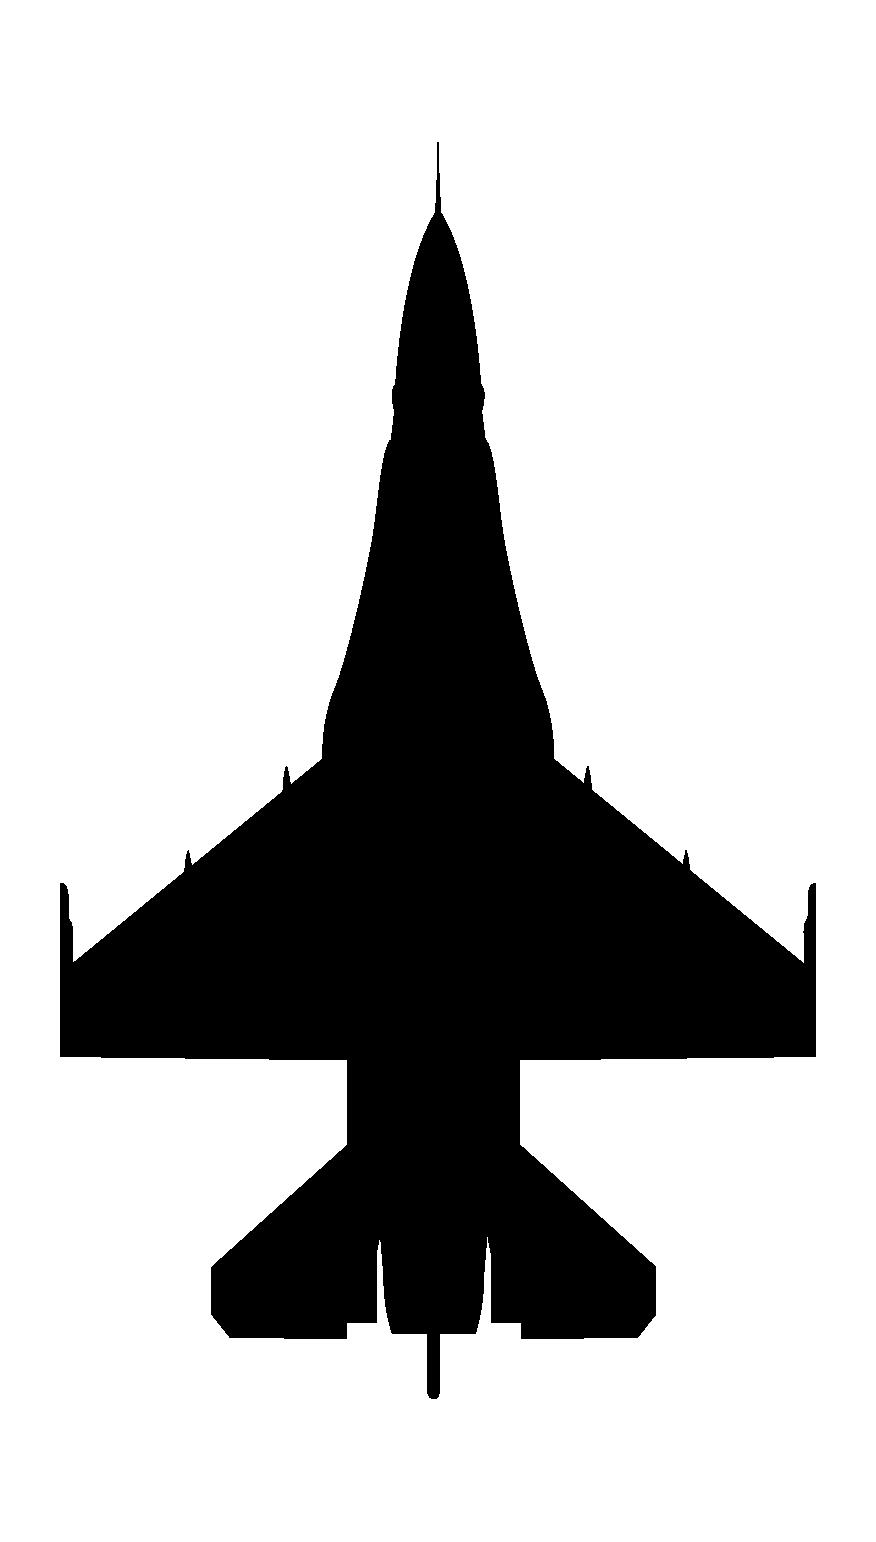
\includegraphics[
                width=5mm,
            ]{diagrams/aircraft/silhouette_f16_top.pdf}
        };
        \node[below] at (approach2)
        {
            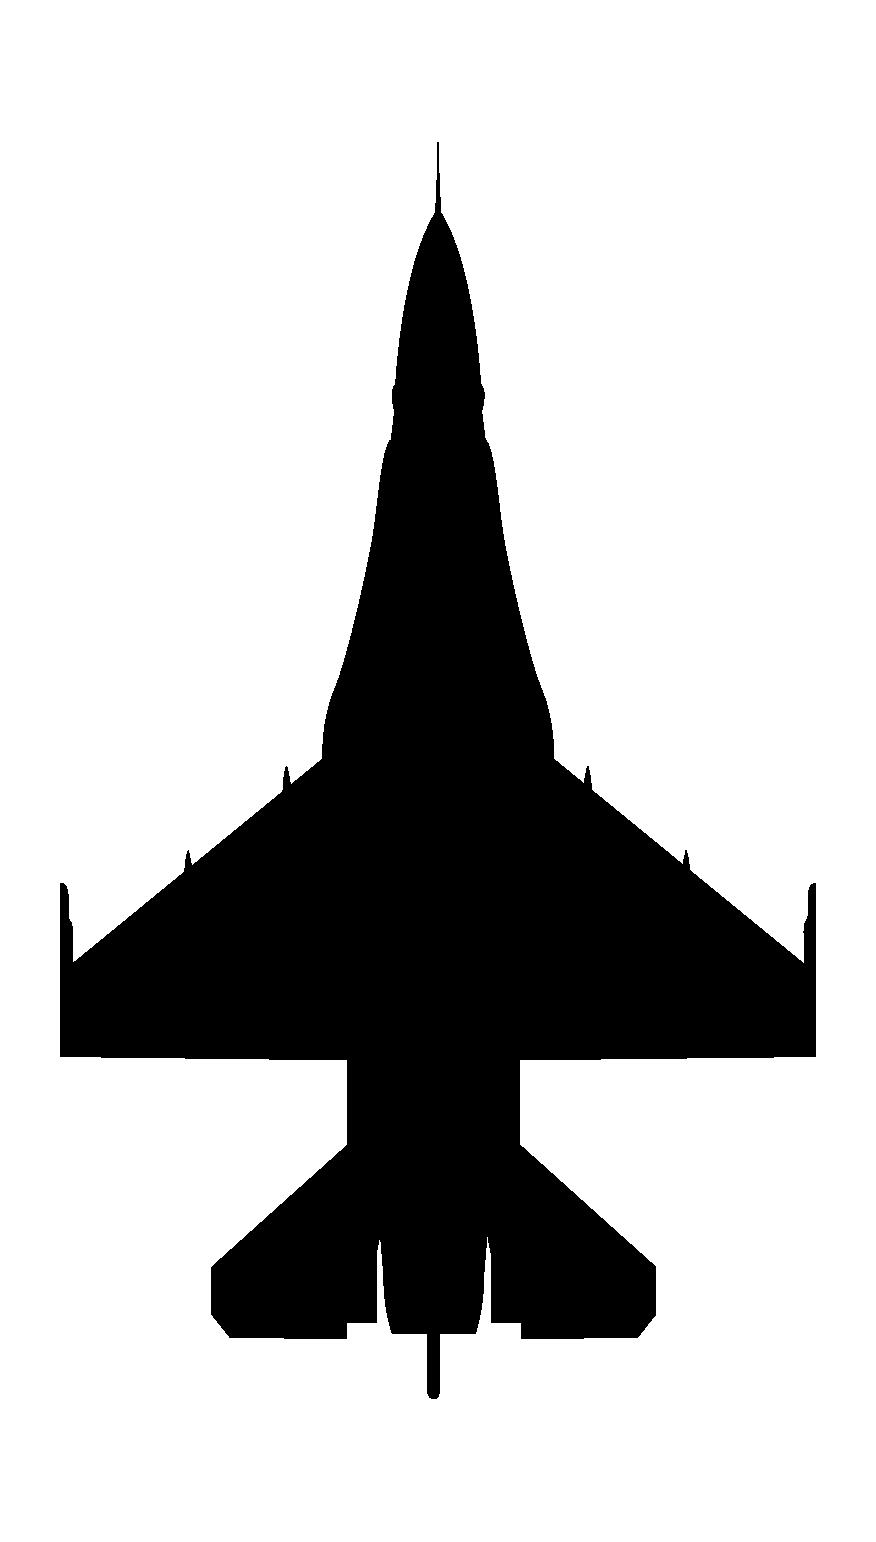
\includegraphics[
                width=5mm,
            ]{diagrams/aircraft/silhouette_f16_top.pdf}
        };
        \node[below] at (approach3)
        {
            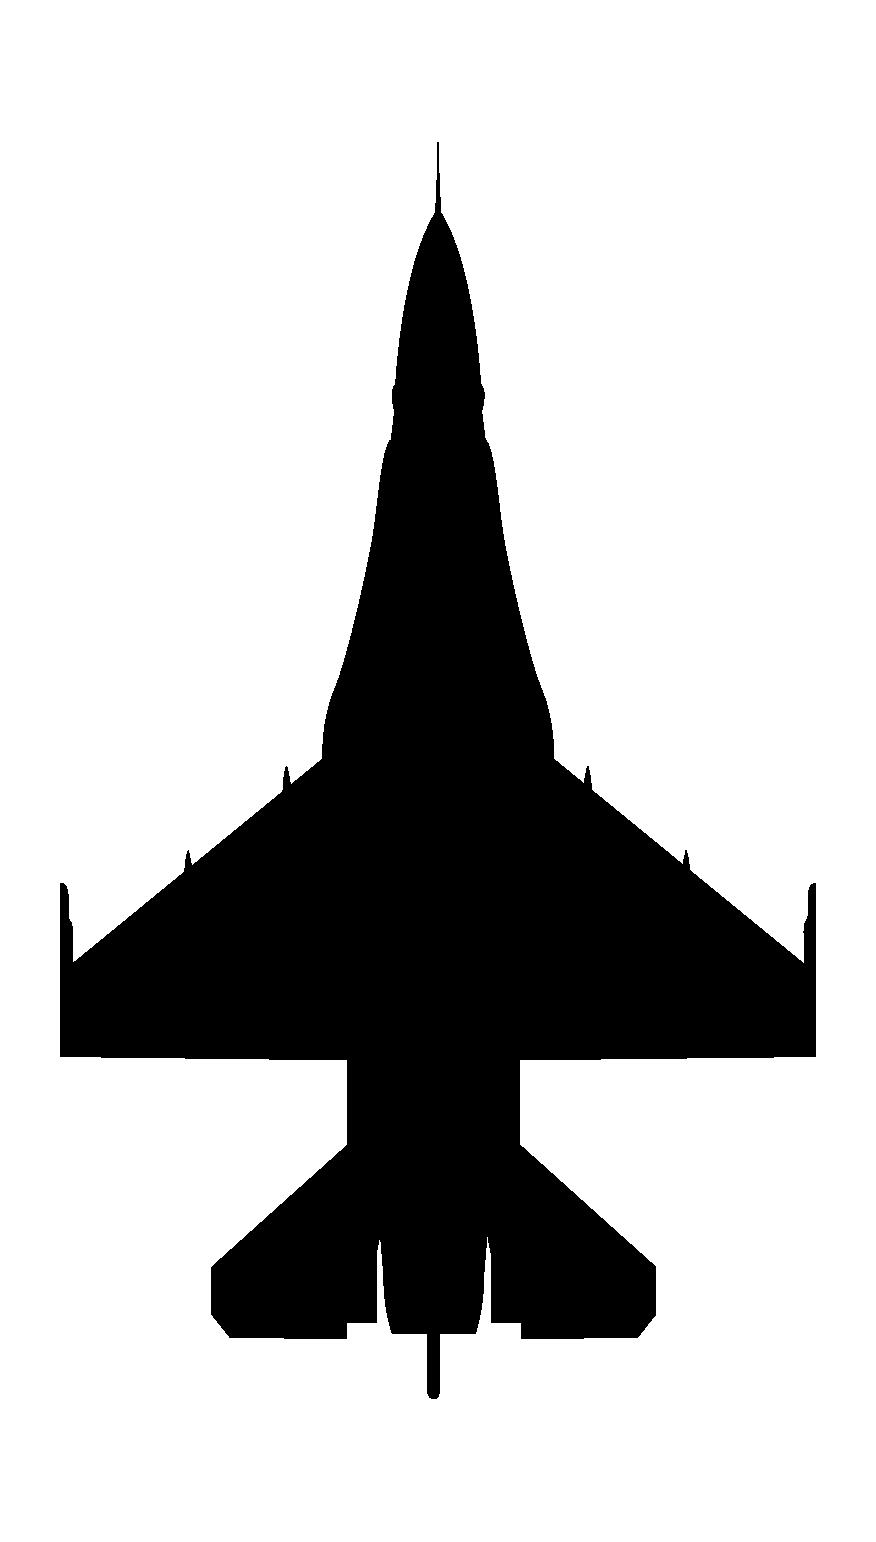
\includegraphics[
                width=5mm,
            ]{diagrams/aircraft/silhouette_f16_top.pdf}
        };
        \node[below] at (approach4)
        {
            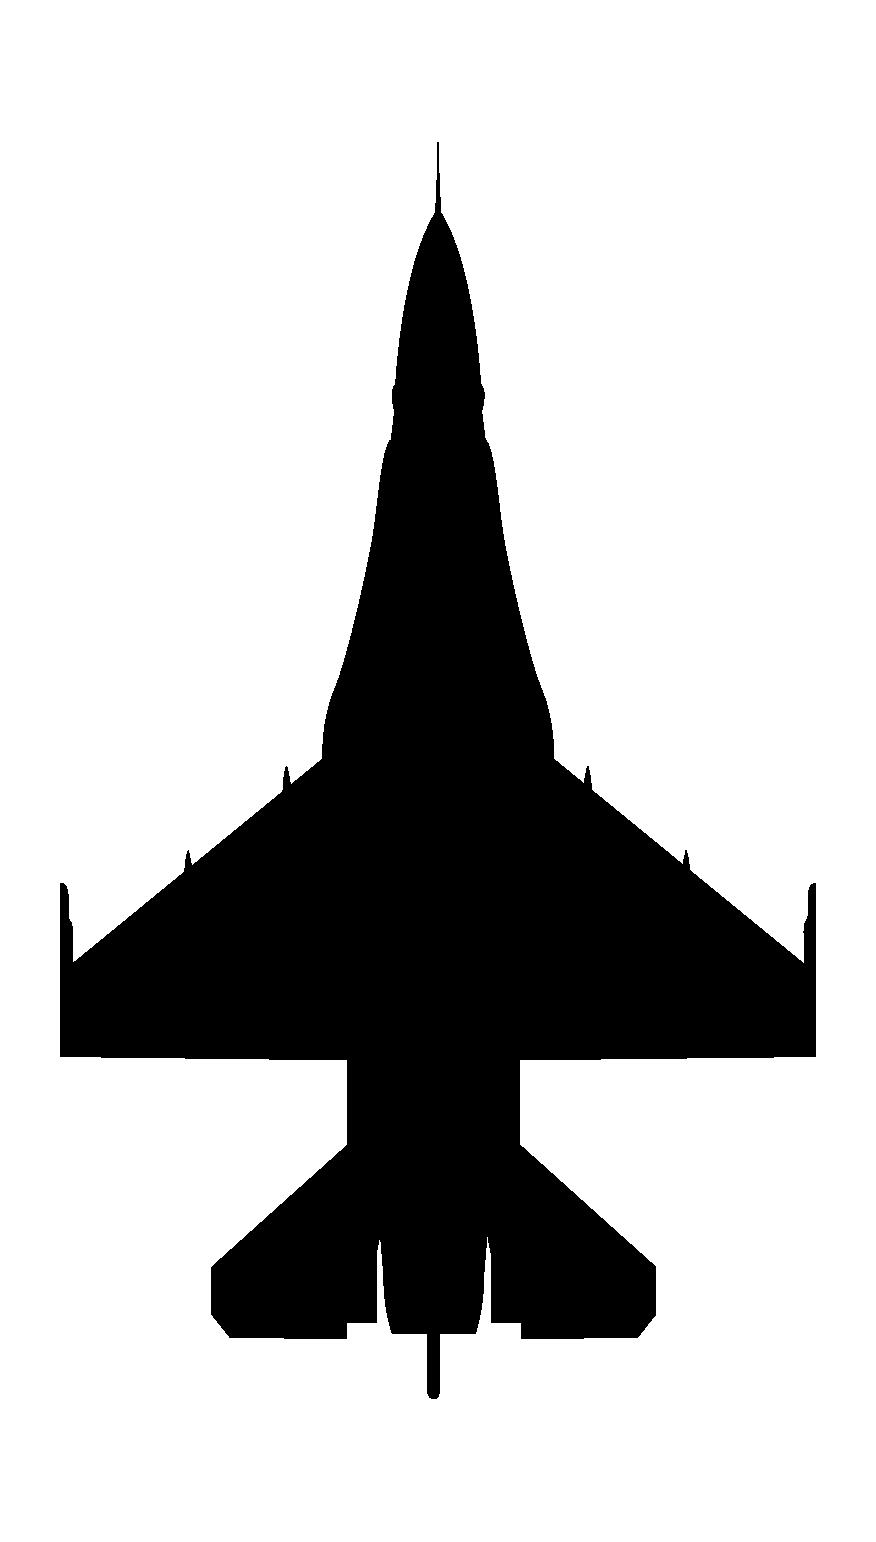
\includegraphics[
                width=5mm,
            ]{diagrams/aircraft/silhouette_f16_top.pdf}
        };

    \end{tikzpicture}
    \caption{Four-ship overhead approach \& break}
    \label{fig:supp_fig:form:overhead}
\end{figure}